%=======================================================================
% English edition preamble — RetNet-272M Technical Report
% Build: xelatex twice
%=======================================================================
\documentclass[11pt,openany]{article}

% Latin text fonts
\usepackage{fontspec}
\setmainfont{Times New Roman}[Ligatures=TeX]
\setsansfont{Microsoft YaHei}
\setmonofont{Consolas}[Scale=0.86]

% CJK fallback for the few Chinese strings that remain (code comments,
% file names, quoted configuration keys).
\usepackage{xeCJK}
\setCJKmainfont{SimSun}[BoldFont=SimHei,ItalicFont=KaiTi]
\setCJKmonofont{FangSong}
\xeCJKsetup{CJKmath=false}

% =====================================================================
%  preamble-common.tex
%  Shared preamble for the RetNet-272M technical report (Chinese and
%  English editions).  Build with XeLaTeX.
%
%  Typographic convention (deliberately plain, single column, as in a
%  conventional technical report):
%    * serif body text, no coloured display headings
%    * numbered tables and figures, each with a caption
%    * remarks set as an indented, labelled passage rather than a
%      coloured box
% =====================================================================

\usepackage{amsmath}
\usepackage{amssymb}
\usepackage{bm}

% ---------- layout ---------------------------------------------------
\usepackage[a4paper,top=2.5cm,bottom=2.5cm,left=2.4cm,right=2.4cm]{geometry}
\usepackage{fancyhdr}
\usepackage{titlesec}
\usepackage{enumitem}
\usepackage{booktabs}
\usepackage{array}
\usepackage{tabularx}
% A table taller than a page must be able to break across pages: an unbreakable
% `tabular` that large is shipped out past the paper edge (Overfull \vbox), and
% the part below the edge is what the reader loses.  `longtable` is used only
% for such tables (see mktex.render_table).
\usepackage{longtable}
\usepackage{ragged2e}
\usepackage{xcolor}
\usepackage{caption}
\usepackage{graphicx}

% ---------- code -----------------------------------------------------
\usepackage{listings}
\usepackage{newunicodechar}

% ---------- references ----------------------------------------------
\usepackage[hidelinks,bookmarksnumbered]{hyperref}
\usepackage{bookmark}

% ---------- colours (used sparingly: code and rules only) ------------
\definecolor{codebg}{RGB}{248,248,249}
\definecolor{codeframe}{RGB}{216,220,225}
\definecolor{codecomment}{RGB}{104,124,108}
\definecolor{codekeyword}{RGB}{0,80,150}
\definecolor{codestring}{RGB}{160,60,40}
\definecolor{rulecol}{RGB}{178,182,188}
\definecolor{headrule}{RGB}{40,48,60}

% ---------- spacing --------------------------------------------------
\linespread{1.04}
\setlength{\parskip}{0.30em}
\setlength{\parindent}{0pt}
\setlength{\abovedisplayskip}{6pt}
\setlength{\belowdisplayskip}{6pt}
\setlength{\abovedisplayshortskip}{4pt}
\setlength{\belowdisplayshortskip}{4pt}

% Mixed CJK / monospace prose has few hyphenation opportunities; give TeX
% more room to stretch instead of leaving overfull boxes.
\tolerance=3000
\emergencystretch=3em
\hyphenpenalty=50
\hbadness=10000

% ---------- headings: plain, black, not coloured ---------------------
\titleformat{\section}
  {\normalfont\large\bfseries}{\thesection}{0.7em}{}
\titleformat{\subsection}
  {\normalfont\normalsize\bfseries}{\thesubsection}{0.7em}{}
\titleformat{\subsubsection}
  {\normalfont\normalsize\itshape}{\thesubsubsection}{0.7em}{}
\titlespacing*{\section}{0pt}{1.5em}{0.55em}
\titlespacing*{\subsection}{0pt}{1.05em}{0.40em}
\titlespacing*{\subsubsection}{0pt}{0.85em}{0.30em}

% ---------- header / footer ------------------------------------------
\pagestyle{fancy}
\fancyhf{}
\renewcommand{\headrulewidth}{0pt}
\renewcommand{\footrulewidth}{0pt}
\fancyfoot[C]{\small\thepage}

% ---------- tables and figures ---------------------------------------
\renewcommand{\arraystretch}{1.18}
\setlength{\tabcolsep}{5pt}
\captionsetup{
  font=small,
  labelfont=bf,
  labelsep=period,
  justification=raggedright,
  singlelinecheck=false,
  skip=5pt,
}
\captionsetup[table]{position=top}
\captionsetup[figure]{position=bottom}

% A numbered table with its caption above, as in the reference report.
\newenvironment{reporttable}[1]
  {\begin{center}\small\captionof{table}{#1}}
  {\end{center}}
\newcommand{\tabnote}[1]{\par\vspace{2pt}{\footnotesize #1}}

% ---------- lists ----------------------------------------------------
\setlist[itemize]{topsep=0.25em,itemsep=0.12em,parsep=0.08em,leftmargin=1.5em}
\setlist[enumerate]{topsep=0.25em,itemsep=0.12em,parsep=0.08em,leftmargin=1.8em}

% ---------- inline code ----------------------------------------------
\newcommand{\code}[1]{\texttt{\small #1}}
\newcommand{\file}[1]{\texttt{\small #1}}

% ---------- code listings --------------------------------------------
\lstdefinestyle{report}{
  backgroundcolor=\color{codebg},
  basicstyle=\ttfamily\fontsize{8.1}{9.6}\selectfont,
  commentstyle=\color{codecomment}\itshape,
  keywordstyle=\color{codekeyword}\bfseries,
  stringstyle=\color{codestring},
  frame=single,
  rulecolor=\color{codeframe},
  framesep=5pt,
  framexleftmargin=5pt,
  xleftmargin=5pt,
  breaklines=true,
  breakatwhitespace=false,
  breakindent=1.2em,
  columns=fullflexible,
  keepspaces=true,
  showstringspaces=false,
  tabsize=4,
  aboveskip=0.6em,
  belowskip=0.6em,
  upquote=true,
  extendedchars=true,
  inputencoding=utf8,
  escapechar=|,
  texcl=false,
  literate=%
    {→}{{$\rightarrow$}}1
    {←}{{$\leftarrow$}}1
    {×}{{$\times$}}1
    {÷}{{$\div$}}1
    {≈}{{$\approx$}}1
    {≤}{{$\leq$}}1
    {≥}{{$\geq$}}1
    {≠}{{$\neq$}}1
    {µ}{{$\mu$}}1
    {γ}{{$\gamma$}}1
    {Δ}{{$\Delta$}}1
    {σ}{{$\sigma$}}1
    {τ}{{$\tau$}}1
    {Σ}{{$\Sigma$}}1
    {√}{{$\surd$}}1
    {·}{{$\cdot$}}1
    {−}{{$-$}}1
    {∈}{{$\in$}}1
    {±}{{$\pm$}}1
    {∞}{{$\infty$}}1
    {❌}{{$\times$}}1
    {✅}{{$\checkmark$}}1
    {⚠}{{!}}1
}
\lstset{style=report}

% `listings` ships no PowerShell dialect; define just enough to colour it.
\lstdefinelanguage{PowerShell}{
  morekeywords={if,else,elseif,foreach,for,while,function,param,return,
    try,catch,finally,switch,break,continue,throw,in,not,and,or},
  sensitive=false,
  morecomment=[l]{\#},
  morestring=[b]",
  morestring=[b]',
}
\lstdefinelanguage{text}{}

% ---------- remarks --------------------------------------------------
% The source uses block quotes for asides.  They are set as an indented
% passage introduced by "Note." rather than as a coloured box.
\newenvironment{notebox}
  {\par\vspace{0.35em}%
   \begin{list}{}{%
     \setlength{\leftmargin}{1.5em}\setlength{\rightmargin}{0.4em}%
     \setlength{\topsep}{0pt}\setlength{\parskip}{0.25em}%
     \setlength{\parsep}{0.25em}\setlength{\itemsep}{0pt}%
     \setlength{\listparindent}{0pt}}%
   \item\relax\textbf{Note.}\ \ignorespaces}
  {\end{list}\vspace{0.15em}}

% ---------- rule -----------------------------------------------------
\newcommand{\reportrule}{\par\vspace{0.5em}{\color{rulecol}\hrule height 0.4pt}\vspace{0.7em}\par}

% ---------- appendices -----------------------------------------------
% The source writes the appendix titles with their letter already in the
% text ("Appendix A: Reproduction"), so the appendix section counter prints
% the letter and the *headings* of the back matter use a second counter that
% renumbers (Reference Reliability Note, References).
\newcounter{backmatter}
\newcommand{\startappendix}{%
  \clearpage
  \setcounter{section}{0}%
  \setcounter{backmatter}{0}%
  \renewcommand{\thesection}{\Alph{section}.}%
  % subsections are numbered against the appendix letter, so pin the format
  % explicitly: leaving \thesubsection as \thesection.\arabic{subsection}
  % would print `B..1' because \thesection already ends in a period.
  \renewcommand{\thesubsection}{\Alph{section}.\arabic{subsection}}%
}
\newcommand{\backmattersection}[1]{%
  \refstepcounter{backmatter}%
  \section*{\arabic{backmatter}.\quad #1}%
  \addcontentsline{toc}{section}{\protect\numberline{\arabic{backmatter}.}#1}%
}


\hypersetup{
  pdftitle  = {RetNet-272M Technical Report},
  pdfauthor = {RetNet Project},
  pdfsubject= {Retentive Networks / Gated Linear Attention / Training Engineering},
  pdfkeywords={RetNet, GLA, chunkwise, torch.compile, mixed precision, single-GPU training},
}

\fancyhead[L]{\small\itshape RetNet-272M Technical Report}
\fancyhead[R]{\small\thepage}
\fancyfoot[C]{}

\begin{document}


%=======================================================================
% English edition title block and abstract -- inserted before the body
%=======================================================================
\thispagestyle{empty}

\begin{center}
\vspace*{3.2cm}

{\LARGE\bfseries A Technical Report on\\[0.25em] Training RetNet-272M}

\vspace{0.55cm}

{\large RetNet-272M Training Technical Report}

\vspace{1.1cm}

{\normalsize RetNet Project}

\vspace{0.25cm}

{\small\itshape 2026-10-11}

\vspace{2.2cm}

\begin{minipage}{0.80\textwidth}
\centering\small
\begin{tabular}{@{}rl@{}}
\toprule
Model & 272.30M parameters, 20 layers, 2048-token context \\
Step time & 2176\,ms $\rightarrow$ 662\,ms ($3.29\times$) \\
Hardware & RTX 4070 Laptop 8\,GB / RTX 3070 8\,GB \\
Data & 552.3\,M-token packed supervised-fine-tuning corpus \\
\bottomrule
\end{tabular}
\end{minipage}

\vfill

{\small\itshape This is the English edition; the Chinese edition is a separate file,
RetNet-272M-Chinese-Report.pdf.}

\vspace{1.2cm}
\end{center}

\clearpage

%-----------------------------------------------------------------------
% Abstract
%-----------------------------------------------------------------------
\section*{Abstract}
\addcontentsline{toc}{section}{Abstract}

We present a technical report on the training of \textbf{RetNet-272M}, a 272.30M-parameter
retentive language model with gated linear attention, trained on a 552.3M-token packed
supervised-fine-tuning corpus at a 2048-token context length on a single 8\,GB consumer
GPU. The report covers:

\begin{enumerate}
\item the architecture, including the multi-scale retention, the learnable per-head decay
      gate, and a function-preserving width-growth layer norm;
\item the data pipeline and its measured composition (7.8 samples per packed row, 2.92\%
      padding, 5.60\% of samples carrying chain-of-thought);
\item a set of \textbf{engineering optimizations that reduce the per-optimization-step time
      from 2176\,ms to 662\,ms ($3.29\times$)} under the real \code{Trainer} path, together
      with kernel-level attribution showing that the residual step splits 66.4\% GEMM /
      33.6\% elementwise and that the GEMM half already runs at or above its
      shape-limited ceiling;
\item a closed-form replacement for the chunkwise state scan that cuts it from 1127\,µs to
      190\,µs per layer while remaining within $10^{-6}$ relative error of the reference
      recurrence; and
\item three \textbf{silent correctness defects} we found and fixed --- a \code{torch.compile}
      state-dict prefix that made every saved checkpoint unloadable, a resume path that had
      never worked, and an equivalence test that compared a function against itself.
\end{enumerate}

We also report negative results: fused linear cross-entropy ($-13\%$ throughput), a
group-norm layout rewrite ($-9.2\%$), \code{max-autotune} compilation (0\%), and physical
batch size 2 (memory-infeasible). Finally, one honest negative result: after controlling for
the benchmark's budget-truncation confound, the 10,000-step continuation scores \textbf{28\%
lower than its own starting point} on the same 242 never-truncated items (0.194 $\rightarrow$
0.141, $\approx 1.6\sigma$), while its stopping behaviour \emph{improved} (truncation
72.5\% $\rightarrow$ 65.2\%, raw think-leak 52.0\% $\rightarrow$ 46.8\%). Our leading ---
\textbf{unverified} --- hypothesis is catastrophic forgetting from restarting a full cosine
schedule on weights already annealed to \code{min\_lr} (peak LR jumps $3.6\times$): the
signature is falling training loss with falling task accuracy.

\bigskip

{\small\textbf{Keywords:} retentive network (RetNet); gated linear attention (GLA); chunkwise
parallelism; closed-form state scan; \code{torch.compile}; 8-bit AdamW; single 8\,GB GPU
training; silent correctness defects.}

\clearpage

%-----------------------------------------------------------------------
% Contents
%-----------------------------------------------------------------------
\renewcommand{\contentsname}{Contents}
\tableofcontents

\clearpage


\section{Introduction}

Our goal is to train a usable Chinese dialogue model end-to-end — pretraining, supervised fine-tuning, evaluation, inference — on a \textbf{single 8 GB consumer GPU}. That constraint drives every design decision: parameter count, context length, optimizer, data packing, and which optimizations are worth attempting.

RetNet is attractive precisely here. It replaces the quadratic attention with a linear recurrence while preserving the property of *one model, three equivalent computations*: chunkwise-parallel for training, parallel for long-sequence prefill, and recurrent for token-by-token decoding. The three forms are mathematically identical, so no separate set of inference weights is needed.

This report does not propose a new architecture. It records the \textbf{complete engineering facts of one model trained to date}: what the architecture is, what the data looks like, where each step's time actually goes, which optimizations really work, and where things were silently wrong. We consider the last category as important as the first: the three correctness defects reported here share a single property — \textbf{none of them raised an error}.

\reportrule

%=======================================================================
%  _supplement.tex -- English prose for the sections that the Markdown
%  source carries only in Chinese.  mktex.py injects this file verbatim
%  between the last English Markdown section and the References list.
%
%  The Chinese-numbered sections 1.--10. supply the \section commands in
%  order, so the numbering below lands automatically:
%     3 Architecture          8 Evaluation
%     4 Data                  9 Limitations and Future Work
%     5 Training Pipeline    10 Conclusion
%     6 Engineering Optimizations
%     7 Correctness Defects
%  followed by Appendices A--D and the reference-reliability note.
%
%  NOTE: Introduction (1) comes from the source's own English prose, which
%  mktex.py does typeset.  Background (2) is re-authored below, because the
%  source's Chinese half of that section would otherwise leak into this
%  edition: its English half is a one-paragraph condensation only.
%=======================================================================

\section{Background}
\label{sec:en-bg}

RetNet [1] replaces attention with \emph{retention}: a causal, exponentially-decayed linear
operator with a parallel form, a recurrent form with an $O(1)$ state
($\approx$ 5.2\,MiB total for the whole 272M model), and a chunkwise form used for
training. Our implementation adopts the \textbf{GLA} [2] parameterisation --- a learnable
per-head $\log\gamma$ --- and the measured gate range is 0.6680--1.0117.

The attraction of retention is threefold. First, the parallel, recurrent and chunkwise
forms compute the same function, so one set of weights serves training, long-sequence
prefill and token-by-token decoding, and no separate inference model has to be maintained.
Second, the recurrent state has a size independent of sequence length: the whole 272M
model's layer states together occupy about 5.2\,MiB, which is what makes inference on an
8\,GB device comfortable. Third, because the decay is a per-head scalar, the gate
parameterisation costs almost nothing in parameters while giving each head an independent
memory horizon.

The measured gate range matters more than it looks. Heads with $\gamma > 1$ \emph{amplify}
history rather than attenuating it, which makes the naive log-space factorisation of the
decay mask overflow in fp32, and it spreads the dynamic range of the state across more than
a dozen orders of magnitude. Several of the numerical hazards discussed later --- the
overflowing intra-chunk mask, the choice of a closed-form scan, and the relative rather
than absolute criterion in the equivalence test --- are direct consequences of that range.

\section{Architecture}
\label{sec:en-arch}

\subsection{Configuration}
\label{sec:en-arch-config}

\begin{center}\small
\captionof{table}{Model configuration}
\begin{tabular}{@{}>{\RaggedRight\arraybackslash}p{0.40\textwidth}>{\RaggedRight\arraybackslash}p{0.52\textwidth}@{}}
\toprule
\textbf{Item} & \textbf{Value} \\
\midrule
Parameters & \textbf{272.30\,M} (272,304,448; reconciled digit by digit against \code{docs/12}) \\
Layers \code{num\_layers} & 20 \\
\code{d\_model} & 1024 \\
\code{num\_heads} & 16 \\
\code{key\_dim} $=$ \code{d\_model}/\code{heads} & 64 \\
\code{value\_dim} & 2048 \\
\code{value\_head\_dim} $=$ \code{value\_dim}/\code{heads} & 128 \\
\code{ffn\_dim} & 2048 \\
\code{vocab\_size} & 20000 \\
\code{use\_swiglu} & false \\
\code{use\_gla} & \textbf{true} \\
\code{use\_growth\_ln} & \textbf{true} (\code{growth\_old\_dim} $=$ 768) \\
\code{tie\_weights} & true (\code{lm\_head} and \code{embedding} are shared) \\
\code{embed\_scale} & 27.712812921102035 $= \sqrt{768}$ \\
\code{norm\_eps} & 1e-5 \\
\code{prompt\_loss\_weight} & 0.1 \\
Context length & 2048 \\
\bottomrule
\end{tabular}
\end{center}

\begin{notebox}
\code{embed\_scale} $= \sqrt{768}$ rather than $\sqrt{1024}$: the model grew from width
768 to width 1024 (Section~\ref{sec:en-arch-growth}), and the scaling factor keeps the
pre-growth width so that the embedding scale stays consistent with early training.
\end{notebox}

\subsection{Multi-Scale Retention}
\label{sec:en-arch-msr}

Each \code{MultiScaleRetention} layer contains five projections
$W_Q, W_K \in \mathbb{R}^{1024 \times 1024}$,
$W_V, W_G \in \mathbb{R}^{1024 \times 2048}$,
$W_O \in \mathbb{R}^{2048 \times 1024}$, one \code{GroupNorm}, and a per-head $\gamma$.
The forward pass is

\[
\begin{aligned}
q, k, v, g &= W_Q x,\ W_K x,\ W_V x,\ W_G x \\
o &= \text{Retention}(q, k, v; \gamma) \\
o &= \text{GroupNorm}(o) \odot \text{SiLU}(g) \\
y &= W_O\, o
\end{aligned}
\]

where the $g$ branch acts as a gate, as in GLA~[2].

\subsection{The Log-Space Decay Mask: A Real Numerical Trap}
\label{sec:en-arch-mask}

The intra-chunk mask needs $\gamma^{\,a-b}$ ($a, b$ are intra-chunk indices). The most
natural way to write it is the \textbf{factorised} form:

\[
\gamma^{\,a-b} = \gamma^{\,a} \cdot \gamma^{-b}
\]

\textbf{This form overflows.} The smallest gate in this model is $\gamma = 0.668$, and
the largest intra-chunk index difference is $C-1 = 255$ (with $C = 256$):

\[
0.668^{-255} \approx 1.0 \times 10^{44} \;>\; 3.4 \times 10^{38} = \text{fp32 maximum}
\]

so the result is $\text{Inf}$ and the forward output is $\text{NaN}$.
\textbf{\code{torch.where} cannot save it} --- it only discards the result, it does not
prevent the $\text{Inf}$ from being computed.

The correct form is \textbf{log-space}:

\[
\text{mask}[a,b] = \exp\!\big(\log \gamma \cdot \max(a-b,\, 0)\big) \cdot \mathbb{1}[a \ge b]
\]

It saturates correctly in both directions: for $\gamma < 1$ the exponent is negative and
it underflows to $0$ (which is where $0$ belongs); for $\gamma > 1$ it gives a finite
value. The $\gamma^{\,a-b}$ of the reference implementation happens to be safe (it can
only underflow, never overflow), but it cannot be batched into a matrix multiplication.

\begin{notebox}
\textbf{Lesson (now written into the code comments).} An equivalence test must cover the
\textbf{real gate range}. The first version of the test used only the default
initialisation ($\gamma \approx 0.97$--$1.0$) and could not detect this $10^{44}$
overflow at all.
\end{notebox}

\subsection{Chunked Recurrence and the Closed-Form Scan}
\label{sec:en-arch-chunk}

\subsubsection{Reference Chunkwise Form}

Let the chunk size be $C$ and the number of chunks $n_c = L/C$, with chunk-level decay
$d_h = \gamma_h^{C}$. Write $S_i$ for the state entering chunk $i$:

\[
\begin{aligned}
U_i &= K_i^{\top}\big(V_i \odot \gamma^{\,C-1-b}\big)
   &&\text{the chunk's contribution to the state} \\
S_{i+1} &= d\, S_i + U_i &&\text{state recurrence} \\
\text{inner}_i &= \big(Q_i K_i^{\top} \odot \text{mask}\big) V_i &&\text{intra-chunk} \\
\text{cross}_i &= \big(Q_i \odot \gamma^{\,a+1}\big) S_i &&\text{inter-chunk}
\end{aligned}
\]

The reference implementation executes the third and fourth lines plus the state
recurrence chunk by chunk, emitting about $3 n_c \approx 97$ mutually dependent small
kernels per layer at $C = 64$.

\subsubsection{The Key Observation}

\textbf{$d$ is constant throughout the loop} (it is the per-head scalar
$d_h = \gamma_h^{C}$, which does not vary with $i$). The recurrence therefore has a
closed form:

\[
S_i \;=\; d^{\,i} S_0 \;+\; \sum_{j<i} d^{\,i-1-j} U_j
\]

Define the matrix $T \in \mathbb{R}^{H \times (n_c+1) \times n_c}$ and the vector
$\tau \in \mathbb{R}^{H \times (n_c+1)}$:

\[
T[h,i,j] = \begin{cases} d_h^{\,i-1-j} & j \le i-1 \\ 0 & j \ge i \end{cases},
\qquad
\tau[h,i] = d_h^{\,i}
\]

Flattening $U$ into
$U_{\text{flat}} \in \mathbb{R}^{B \times H \times n_c \times (d_k d_v)}$, \textbf{one
batched matrix multiplication} produces every historical state:

\[
S_{\text{all}} = T\, U_{\text{flat}} \;+\; \tau \odot S_0
\;\in\; \mathbb{R}^{B \times H \times (n_c+1) \times (d_k d_v)}
\]

The first $n_c$ rows are exactly $\{S_0, S_1, \dots, S_{n_c-1}\}$, and \textbf{row $n_c$
is exactly the new post-recurrence state} $S_{n_c}$ --- no extra recurrence step is
needed.

\textbf{Numerical safety.} Every exponent of $T$, $i-1-j \ge 0$, is \textbf{non-negative},
so the $\gamma^{-j}$ overflow of Section~\ref{sec:en-arch-mask} cannot occur here.
However small $d$ is, it can only underflow to $0$, and that correctly means ``the history
has been forgotten''.

\textbf{Cost analysis.} The FLOPs rise from $O(n_c H d_k d_v)$ to $O(n_c^2 H d_k d_v)$
--- at $C = 128$ ($n_c = 16$) that is $17 \times 16 \times 8192 \times 16 \approx
3.6 \times 10^7$ MAC, i.e.\ 71 MFLOP, entirely negligible against the 3.46 TFLOP of GEMM
per micro-step. What is bought is the \textbf{kernel launch count}: 97 $\rightarrow$
about 5.

\textbf{Measured} (eager, one layer, $C = 64$, $n_c = 32$):

\begin{center}\small
\captionof{table}{Per-layer cost of the closed-form scan}
\begin{tabular}{@{}lrr@{}}
\toprule
\textbf{Implementation} & \textbf{Per-layer time} & \textbf{$\times$ 20 layers} \\
\midrule
Chunk-by-chunk loop $+$ \code{torch.stack} & \textbf{1127.5\,$\mu$s} & 22.6\,ms/micro-step \\
Closed-form batched matmul & \textbf{190.5\,$\mu$s} & 3.8\,ms/micro-step \\
\bottomrule
\end{tabular}
\end{center}

\textbf{Equivalence.} Against the reference recurrence it is \textbf{bit-identical} for
$\gamma \le 0.85$; for $\gamma \ge 1$ there is a 1--3\% relative difference whose source
is a different rounding path --- the old form multiplies the bf16 $d$ sixteen times in a
row (accumulated error $\approx 15 \times 2^{-8} \approx 6\%$), while the new form computes
$d^k$ in fp32 and converts once ($\approx 0.4\%$). \textbf{Both are at the level of fp32
accumulation-order noise, and the new form is the more accurate of the two.} With the
criterion fixed, all 15 combinations in \code{tests/test\_fast\_chunkwise.py} pass
(relative error $\sim 10^{-6}$).

\subsection{An Equivalent Form of GroupNorm}
\label{sec:en-arch-gn}

\code{MultiScaleRetention} uses \code{nn.GroupNorm(num\_groups=H, num\_channels=value\_dim)}
applied to $[B{\cdot}L,\ H{\cdot}v_{hd},\ 1]$. Because \textbf{the number of groups equals
the number of heads} and the spatial dimension is 1, each group is exactly the $v_{hd}$
channels of one head, so the operator is \textbf{equivalent} to a LayerNorm along the last
dimension for each $(b,h,l)$ (biased variance, the same $\varepsilon$), with the affine
coefficients grouped per head:

\[
y[b,h,l,j] = \frac{x[b,h,l,j]-\mu_{b,h,l}}{\sqrt{\sigma^2_{b,h,l}+\varepsilon}}
\;\cdot\; w[h{\cdot}v_{hd}+j] \;+\; b[h{\cdot}v_{hd}+j]
\]

We tried rewriting the operator on that basis as ``normalise first, then permute once at
the end'', in order to remove the reference implementation's intermediate copy.
\textbf{It measured 9.2\% \emph{slower}} (190 vs 174\,ms per micro-step): the reference
implementation puts the permute \emph{before} the normalisation, so that copy is
immediately absorbed by the elementwise normalisation kernel; moving it \emph{after}
makes it the input of \code{out\_proj} (an external cuBLAS call), where it can no longer
be fused into anything. \textbf{Reverted}; the test stays in
\code{tests/test\_head\_group\_norm.py}.

\subsection{Function-Preserving Width Growth (GrowthLayerNorm)}
\label{sec:en-arch-growth}

The 768 $\rightarrow$ 1024 width growth of this model relies on a two-segment LayerNorm.
Let the old dimension be $d_o$, the new dimension $d_n$, and the total
$d = d_o + d_n$:

\[
\text{LN}_{\text{grow}}(x) =
\big[\,\text{LN}_{\text{old}}(x_{1:d_o}) \,\big\|\, \gamma_{\text{new}} \odot x_{d_o+1:d} + \beta_{\text{new}} \,\big]
\]

With the initialisation $\gamma_{\text{new}} = 0,\ \beta_{\text{new}} = 0$, the output of
the new channels is \textbf{identically 0}, so the residual branch of that layer is
\textbf{bit-identical at the instant of growth} --- this is strict function-preserving
initialisation (FPI) in its LayerNorm form.

The key point is that \textbf{the statistics of the old channels are not affected by the
new ones}: if a standard LayerNorm is applied directly to the concatenated
$d$-dimensional vector, both $\mu$ and $\sigma$ are polluted by the new channels. Writing
it in two segments decouples the two.

\subsection{Loss}
\label{sec:en-arch-loss}

Weighted by the weight code $w \in \{0, 0.1, 1\}$ and self-normalising:

\[
\mathcal{L} = \frac{\sum_{i} w_i \cdot \text{CE}\big(\text{logits}_i,\ y_i\big)}{\sum_i w_i},
\qquad
w_i = \begin{cases}
0 & \text{padding} \\
1 & \text{assistant reply / plain text} \\
0.1 & \text{prompt}
\end{cases}
\]

The prompt weight is 0.1 so that the model conditions on the user input without spending
generation capacity on repeating the question.

\section{Data}
\label{sec:en-data}

\subsection{Measured Composition}
\label{sec:en-data-composition}

A full read-only scan of \code{data\_cache/chat\_pack\_v13/train.ids.npy}
(269,561 $\times$ 2049) together with \code{train.wcode.npy} gives:

\begin{center}\small
\captionof{table}{Measured composition of the packed corpus}
\begin{tabular}{@{}>{\RaggedRight\arraybackslash}p{0.34\textwidth}>{\RaggedRight\arraybackslash}p{0.58\textwidth}@{}}
\toprule
\textbf{Quantity} & \textbf{Measured} \\
\midrule
Rows $\times$ width & 269,561 $\times$ 2049 \\
Total token slots & \textbf{552,330,489} \\
Padding (wcode $=$ 0) & 16,126,035 (\textbf{2.92\%}) \\
Weight-code distribution & reply 358,896,326 / prompt 144,461,792 / plain 32,846,336 \\
Samples (\code{<bos>} count) & \textbf{2,107,335} (7.8 per row on average) \\
Rows with \code{<think>} / rows with \code{</think>} & 80,504 / 69,199 (row-level closure \textbf{86.0\%}) \\
\code{<think>} occurrences / \code{</think>} occurrences & 123,604 / 100,040 (occurrence-level closure \textbf{80.9\%}) \\
Share of samples carrying \code{<think>} & \textbf{117,973 / 2,107,335 $=$ 5.60\%} \\
\bottomrule
\end{tabular}
\end{center}

\subsection{Conversation Encoding}
\label{sec:en-data-encoding}

\code{retnet/chat.py} is the single implementation \textbf{shared} by data construction and
inference, which guarantees that the boundaries agree:

\begin{lstlisting}[language=]
<bos> [设定：<persona>\n] 用户：U1\n助手：<think>R1</think>A1 [\n用户：U2\n助手：…] <eos>
\end{lstlisting}

\code{<think>} $=$ \code{[5690, 533, 2605, 33]} and \code{</think>} $=$
\code{[5690, 18, 533, 2605, 33]} --- \textbf{differing by exactly one token}
(id 18 $=$ \code{/}). Decoded id by id: \code{5690='<'}, \code{533='th'},
\code{2605='ink'}, \code{33='>'}, \code{18='/'}.

Three corollaries:

\begin{enumerate}
\item \textbf{Closure is a binary decision to insert one token at one position}, and is
      therefore intrinsically capacity-independent.
\item They are \textbf{ordinary BPE tokens, not registered special tokens}, so
      \code{skip\_special\_tokens=True} does not strip them and a leak is visible text in
      the decoded output.
\item \code{<} $=$ 5690 (no leading space) and 19965 (\code{ >} with a leading space) are
      \textbf{different tokens}; the same holds for \code{/} $=$ 18 and 1788. A
      character-level criterion must therefore be written on ids, not on strings.
\end{enumerate}

\subsection{Side Effects of Packing}
\label{sec:en-data-packing}

\code{build\_chat\_mix\_v13.py} is \code{concat([v9 re-cut rows, newly encoded rows])},
with the boundary at $269{,}192{,}388 // 2049 = 131{,}377$ rows:

\begin{itemize}
\item base region: 131,377 rows, \textbf{padding $=$ 0};
\item newly encoded region: 138,184 rows, \textbf{padding $=$ 16,126,035 (5.7\%)} --- all
      of the padding lives here.
\end{itemize}

The mechanism: a truncated sample is exactly 2048 tokens long, so it can only occupy a row
of its own; best-fit packing has nothing that fits beside it. The cost is 16.1M slots
(2.9\% of the whole pack) thrown away --- they carry $w = 0$, so they do not enter the
loss, but they do occupy context window.

\section{Training Pipeline}
\label{sec:en-pipe}

\subsection{Configuration}
\label{sec:en-pipe-config}

\begin{center}\small
\captionof{table}{Training configuration}
\begin{tabular}{@{}>{\RaggedRight\arraybackslash}p{0.26\textwidth}>{\RaggedRight\arraybackslash}p{0.24\textwidth}>{\RaggedRight\arraybackslash}p{0.42\textwidth}@{}}
\toprule
\textbf{Item} & \textbf{Value} & \textbf{Note} \\
\midrule
\code{batch\_size} & 1 & physical batch, limited by the 8\,GB card \\
\code{grad\_accum} & 4 & effective batch 4 $=$ 8192 tokens/optimization step \\
\code{chunk\_size} & 64 (first leg) / \textbf{128} (second leg) & see Section~\ref{sec:en-eng-dead} \\
\code{max\_steps} & 50,000 & optimization steps \\
\code{lr} $\rightarrow$ \code{min\_lr} & 4e-5 $\rightarrow$ 4e-6 & \code{cosine\_with\_min\_lr} \\
\code{warmup} & 500 & \\
\code{optim} & \code{adamw\_bnb\_8bit} & 8-bit AdamW [11] \\
\code{precision} & bf16 & \\
\code{grad\_checkpoint} & \textbf{false} & turning it off saves 1/3 of the step time, at the cost of resident activations \\
\code{compile} & \textbf{true} & \code{torch.compile(inductor)}, see Section~\ref{sec:en-eng-compile} \\
\code{save\_steps} / \code{eval\_steps} & 2500 / 2500 & \\
\code{eval\_batch\_mult} & 4 (first leg) $\rightarrow$ \textbf{1} (second leg) & see Section~\ref{sec:en-eng-dead} \\
\code{auto\_restart\_max} & 3 & see Section~\ref{sec:en-def-resume} \\
\bottomrule
\end{tabular}
\end{center}

\subsection{Training Legs}

\begin{figure}[htbp]
\centering
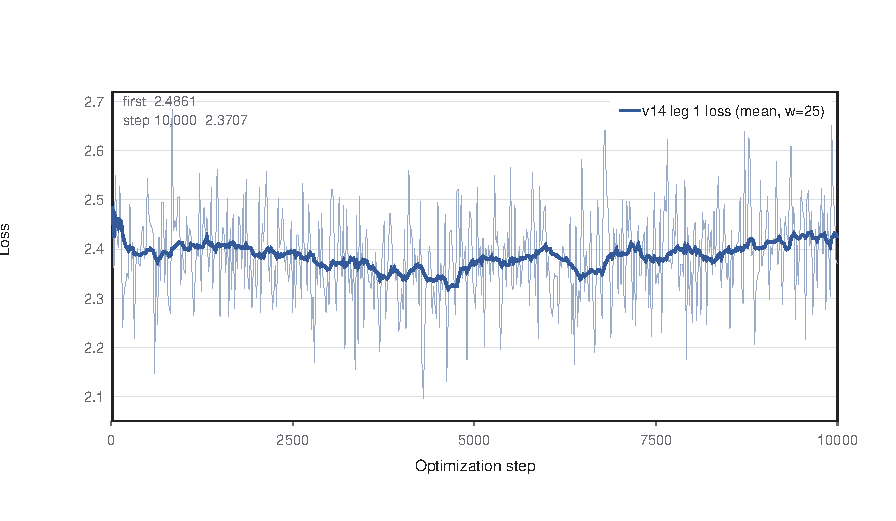
\includegraphics[width=\linewidth]{../figures/fig-loss}
\caption{Training loss of v14 leg 1 (light: per-step, dark: 25-step rolling mean). Measured $2.4861 \rightarrow 2.3707$.}
\label{fig:fig-loss}
\end{figure}

\begin{figure}[htbp]
\centering
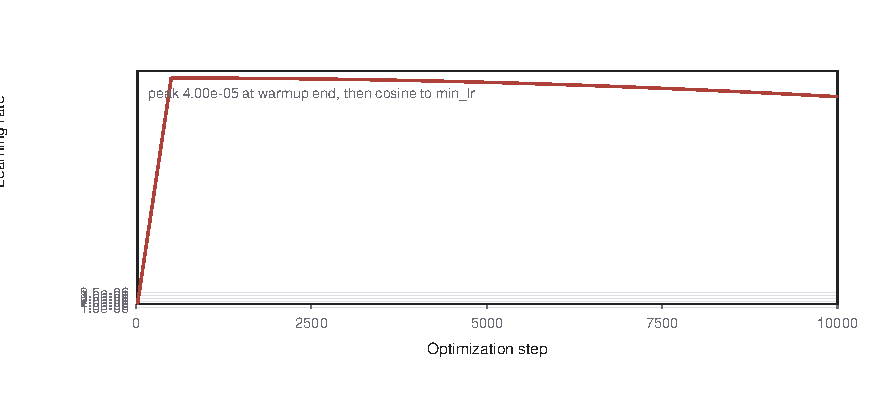
\includegraphics[width=\linewidth]{../figures/fig-lr}
\caption{Learning-rate schedule over the same interval: warmup to a peak of $1.52\times10^{-6}$, then cosine decay.}
\label{fig:fig-lr}
\end{figure}
\label{sec:en-pipe-legs}

\begin{center}\small
\captionof{table}{Training legs}
\begin{tabular}{@{}>{\RaggedRight\arraybackslash}p{0.14\textwidth}>{\RaggedRight\arraybackslash}p{0.16\textwidth}>{\RaggedRight\arraybackslash}p{0.13\textwidth}>{\RaggedRight\arraybackslash}p{0.47\textwidth}@{}}
\toprule
\textbf{Leg} & \textbf{Step range} & \textbf{Status} & \textbf{Note} \\
\midrule
First leg & 0 $\rightarrow$ 10,101 & completed & continuation exported from v13; \code{chunk\_size} was in fact 64 \\
Second leg & 10,000 $\rightarrow$ 50,000 & \textbf{in progress} & continuation from \code{checkpoint-10000}, \code{chunk\_size=128} \\
\bottomrule
\end{tabular}
\end{center}

The first leg's measured loss (recorded every 20 steps) falls from \textbf{2.4861} to
\textbf{2.3707}; the last \code{learning\_rate = 3.6827e-05} agrees exactly with the
configured cosine schedule's \textbf{theoretical value 3.68e-05 at step 10100}, which shows
that both the scheduler and the progress accounting are correct.

The second leg (the continuation, \code{chunk\_size=128}) reproduces the same behaviour over
the same interval:

\begin{lstlisting}[language=]
首条  {'loss': 2.4092, 'grad_norm': 2.739, 'learning_rate': 3.681386e-05, 'epoch': 0.15}
末条  {'loss': 2.3686, 'grad_norm': 3.412, 'learning_rate': 3.574538e-05, 'epoch': 0.17}
\end{lstlisting}

The LR falls monotonically from 3.6814e-05 to 3.5745e-05, \textbf{exactly the trajectory
cosine should follow}; the loss fluctuates between 2.23 and 2.68, the same range as the
first leg over the same interval. This simultaneously verifies that \textbf{the optimizer
state, the LR-scheduler state and the global step count are all restored correctly by HF}.

\begin{notebox}
There is one unexplained observation: the first leg's loss near step 10020 is about 2.47,
while the second leg at the same position is 2.4092 --- a gap of about 0.06, far larger than
the measured chunk-64/128 single-batch difference of 2.4e-7 reported in
Section~\ref{sec:en-eng-dead}. The second leg was rolled back to \code{checkpoint-10000} and
rerun (the 101 steps 10001--10101 of the first leg were discarded), so the two should have
seen the same data window. \textbf{We did not get to the bottom of this}; it is listed as an
open item in Section~\ref{sec:en-limits}.
\end{notebox}

\subsection{A Silent Correctness Bug We Stepped On: HF's Loss Normalisation}
\label{sec:en-pipe-lossbug}

The trailing \code{**\_kwargs} in the signature of \code{RetNetForCausalLM.forward} makes
HF's heuristic infer \code{accepts\_loss\_kwargs = True}, and
\code{Trainer.training\_step} therefore \textbf{skips}

\begin{lstlisting}[language=Python]
loss = loss / self.current_gradient_accumulation_steps
\end{lstlisting}

while this model's loss is already self-normalised by $\sum w$ (it does not use
\code{num\_items\_in\_batch}). The consequence is that \textbf{the gradients are inflated by
a factor of \code{accum} and the effective learning rate rises by the same factor} ---
silently, and only when \code{accum > 1}. The measured symptom was the loss going from 3.19
to \textbf{12.75 $\approx$ 3.19 $\times$ 4}. The fix is to declare it explicitly on the model
class:

\begin{lstlisting}[language=Python]
accepts_loss_kwargs = False     # note: the attribute name has no model_ prefix
\end{lstlisting}

After the fix the loss immediately returns to 3.1851 $\rightarrow$ 3.0148, consistent with
3.20 $\rightarrow$ 3.17 at a real batch of 4.

\begin{notebox}
Every previous task in this project used \code{accum = 1}, so this mine was never stepped
on. \textbf{The moment gradient accumulation is enabled it has to be fixed first.}
\end{notebox}

\section{Engineering Optimizations}
\label{sec:en-eng}

\subsection{Measurement Methodology}
\label{sec:en-eng-method}

All step times are measured with \code{scripts/bench\_trainer.py}, which \textbf{replicates}
the entire path of \code{run\_task.py} (same model construction, same
\code{TrainingArguments}, same dataset object, same collator), discards the first 25 steps
(including inductor's first compilation), and takes \textbf{four times the median
micro-step} as the optimization-step time.

Three disciplines, each of which was bought with a mistake:

\begin{enumerate}
\item \textbf{Wall clock rules everything.} The profiler's \textbf{operator attribution
      misleads}: it credited \code{NativeDropoutBackward0} with 25\%, while actually turning
      dropout off saved only 3.9\%.
\item \textbf{The power source must always be stated.} The same configuration is about
      40\% slower on battery; an early ``5.9\% rotary-cache gain'' was a phantom measured
      that way. Every number in this report was measured at
      \code{BatteryStatus=2} (AC).
\item \textbf{Never tune the algorithm without watching memory.} Disabling gradient
      checkpointing while memory has not been freed causes thrashing and presents as ``the
      algorithm got slower'' --- the same configuration was measured at 1437\,ms and then at
      183\,ms purely as a result of memory.
\end{enumerate}

\subsection{Results}
\label{sec:en-eng-results}

\begin{center}\small
\captionof{table}{Optimization step time and throughput by configuration}
\begin{tabular}{@{}>{\RaggedRight\arraybackslash}p{0.48\textwidth}rrr@{}}
\toprule
\textbf{Configuration} & \textbf{Step time} & \textbf{Throughput} & \textbf{vs A} \\
\midrule
\textbf{A} reference: chunk loop, chunk 64, batch 4, gradient checkpointing, no compile
  & 2176\,ms & 3764 tok/s & 1.00$\times$ \\
\textbf{B} batched chunkwise $+$ \code{torch.compile}, batch 4, gradient checkpointing
  & 903\,ms & 8814 tok/s & \textbf{2.41$\times$} \\
\textbf{C} $=$ B $+$ batch1$\times$accum4 $+$ no gradient checkpointing $+$ 8-bit AdamW
  & 713\,ms & 11496 tok/s & \textbf{3.05$\times$} \\
\textbf{C$'$} $=$ C $+$ closed-form scan $+$ decay-table reuse (this report)
  & \textbf{662\,ms} & \textbf{12373 tok/s} & \textbf{3.29$\times$} \\
\bottomrule
\end{tabular}
\end{center}

C$'$ is \textbf{1.36$\times$} relative to B and 1.08$\times$ relative to C. Three repeat
measurements: 657 / 662 / 663\,ms, jitter $<1\%$.

\textbf{The mechanism of each step:}

\begin{itemize}
\item \textbf{A $\rightarrow$ B (2.41$\times$)}: the four small matmuls per chunk ($C = 64$
      means 128 per layer per step, 9241 \code{aten::matmul} model-wide) become three
      cross-chunk batched matmuls plus one small state scan, dropping the number of
      \code{matmul} calls to 441.
\item \textbf{B $\rightarrow$ C (1.26$\times$)}: gradient checkpointing adds a whole extra
      forward pass --- forward once $+$ recompute once $+$ backward once $=$ 3 passes
      instead of 2 --- so \textbf{a full 1/3 of the step time is recomputation}. Removing it
      requires freeing memory first: 8-bit AdamW compresses the optimizer state from
      2.18\,GiB to 0.55\,GiB, and \code{batch 1 $\times$ accum 4} cuts the activations to a
      quarter.
\item \textbf{C $\rightarrow$ C$'$ (1.08$\times$)}: see Section~\ref{sec:en-arch-chunk}.
\end{itemize}

\subsection{Kernel-Level Attribution}

\begin{figure}[htbp]
\centering
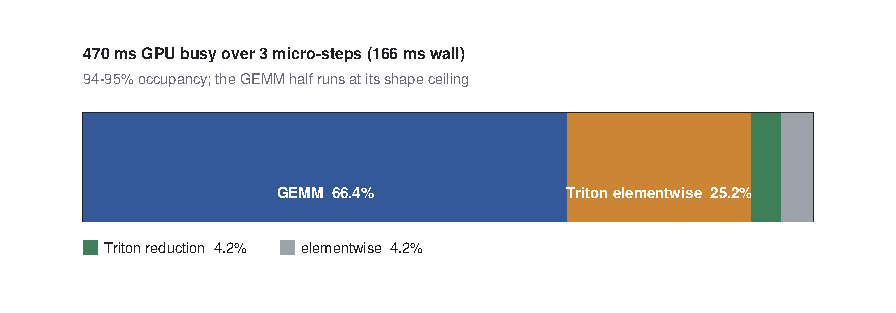
\includegraphics[width=\linewidth]{../figures/fig-kernels}
\caption{GPU busy time aggregated by CUDA kernel class over three micro-steps at C$'$.}
\label{fig:fig-kernels}
\end{figure}
\label{sec:en-eng-kernels}

After exporting a chrome trace, \code{scripts/profile\_kernels.py} aggregates \textbf{by CUDA
kernel} rather than by operator. The sample below covers 3 micro-steps under C$'$:

\begin{center}\small
\captionof{table}{Kernel-level busy time at C$'$ (three micro-steps)}
\begin{tabular}{@{}>{\RaggedRight\arraybackslash}p{0.30\textwidth}rrrr@{}}
\toprule
\textbf{Category} & \textbf{Busy time} & \textbf{Share} & \textbf{Kernels} & \textbf{Mean} \\
\midrule
GEMM & 312\,ms & \textbf{66.4\%} & 2169 & 143.8\,$\mu$s \\
Triton elementwise & 118\,ms & 25.2\% & 3462 & 34.1\,$\mu$s \\
Triton reduction & 20\,ms & 4.2\% & 555 & 35.6\,$\mu$s \\
\code{elementwise} & 20\,ms & 4.2\% & 762 & 25.7\,$\mu$s \\
\bottomrule
\end{tabular}
\end{center}

\textbf{Total busy time 470\,ms / 3 micro-steps $=$ 157\,ms against 166\,ms of wall clock
$=$ 94--95\% occupancy.}

\begin{notebox}
\textbf{An old conclusion that has been overturned.} The project previously used ``GPU busy
time / wall clock'' to declare configuration C to be \textbf{20.8\% idle}, and concluded from
that that ``removing kernels is useless''. That figure was measured \textbf{on battery}. On
AC the true occupancy is \textbf{94\%} --- the premise is false and the conclusion ``removing
kernels is useless'' collapses with it. In fact both optimizations in this report
(Section~\ref{sec:en-arch-chunk} and Section~\ref{sec:en-eng-decay}) are kernel removal, and
together they recover 8\%.
\end{notebox}

\subsection{Launch-Count Optimization of the Decay Tables}
\label{sec:en-eng-decay}

\code{\_decay\_tables} builds the intra-chunk mask and three 1-D decay tables for every
layer. It handles only 260{,}000 elements, yet it costs \textbf{410\,$\mu$s} --- almost all
of it \textbf{launch latency}: about 22 mutually dependent small kernels at roughly 18\,$\mu$s
per launch on Windows.

The goal is therefore not ``compute less'' but ``launch less'':

\begin{enumerate}
\item cache the index tensors (\code{arange}/\code{sub}/\code{ge}/\code{clamp}), saving 4
      launches;
\item reuse one $\gamma^{\,j}$ table ($[H,C]$) for all three 1-D tables:
      $\text{cross} = \gamma^{\,j} \cdot \gamma$,
      $\text{value} = \text{flip}(\gamma^{\,j})$,
      $\text{chunk} = \gamma^{\,j}[-1] \cdot \gamma$, compressing 3 \code{exp} calls into 1.
\end{enumerate}

\textbf{Effect}: the 469\,$\mu$s reduction kernel that used to hold a Top-18 slot
(\code{triton\_red\_fused\_\_to\_copy\_add\_exp\_%
\allowbreak log\_mul\_select\_sum\_view\_zeros})
\textbf{disappears from the list}, and Triton-reduction busy time drops \textbf{47 $\rightarrow$
20\,ms}.

\subsection{Fixing Two Silent \code{torch.compile} Failures}
\label{sec:en-eng-compile}

Before 2026-10-10, \code{torch.compile} was \textbf{completely ineffective} in this project:
measured 0.0\%. There were two independent reasons:

\begin{enumerate}
\item \textbf{No Triton.} The laptop's conda environment was missing \code{triton-windows}.
      Inductor compiles \textbf{lazily}, so \code{TritonMissing} is raised only at the first
      forward pass --- long after \code{train.py}'s \code{try} block has been left --- and it
      therefore \textbf{neither crashes nor speeds anything up: it silently does nothing}.
\item \textbf{The compiled model was never called.} \code{Trainer.\_\_init\_\_} stores the
      \textbf{original} model in \code{self.model\_wrapped}, while \code{train()} takes
      \code{self.\_wrap\_model(self.model\_wrapped)}. Replacing only \code{trainer.model}
      means the compiled model is never invoked: the log says
      \code{torch.compile applied}, the dynamo counters are empty, and the speed does not
      change at all (it was in fact 1.8$\times$ \emph{slower} because of
      \code{OptimizedModule}'s attribute forwarding).
\end{enumerate}

After the fix the dynamo counters show
\code{\{'frames': \{'total': 1, 'ok': 1\}, 'unique\_graphs': 1\}} --- \textbf{one whole graph
captured}.

\begin{notebox}
But it was exactly this fix --- replacing both attributes at once --- that introduced the far
more serious prefix defect of Section~\ref{sec:en-def-prefix}. The final solution is given
there: \textbf{replace \code{forward} in place} instead of wrapping the module.
\end{notebox}

\subsection{Three Dead Config Fields}
\label{sec:en-eng-dead}

\textbf{\code{config.chunk\_size} was always a dead field.} In the signature of
\code{RetNetForCausalLM.forward}, \code{chunk\_size=64} is a \textbf{function default}, the
HF Trainer \textbf{never} passes that keyword when it calls the model, and \code{forward}
\textbf{never reads} \code{self.config.chunk\_size} (it only
\code{getattr(self.config,"mode")}). Measured:

\begin{lstlisting}[language=]
config.chunk_size = 64 / 128 / 256  ->  loss all 2.69759822   (bit-identical = config ignored)
explicit chunk_size = 128           ->  loss 2.69759798       (the parameter itself is live)
\end{lstlisting}

\textbf{So the project always ran at chunk 64 while the task JSON, the logs and the docs all
said 128.} The \code{--sweep chunk\_size=32,64,128,256} of \code{bench\_step.py} swept a
variable that did nothing, and the sentence in \code{docs/15} \S6 --- ``chunk 512/1024 is
actually slower, the optimum is 128'' --- \textbf{does not hold}.

The \textbf{first valid chunk sweep}, after the fix:

\begin{center}\small
\captionof{table}{Chunk-size sweep}
\begin{tabular}{@{}rrr@{}}
\toprule
\textbf{chunk} & \textbf{Step time} & \textbf{reserved} \\
\midrule
64 & 663\,ms & 6.73\,GiB \\
\textbf{128} & \textbf{662\,ms} & \textbf{6.61\,GiB} \\
256 & 685\,ms & 6.90\,GiB \\
\bottomrule
\end{tabular}
\end{center}

\textbf{64 and 128 tie; 256 is 3.5\% slower} --- chunk size is a pipeline-correctness issue,
not a performance lever.

\textbf{\code{eval\_batch\_mult} was dead too}: the configuration template of
\code{run\_task.py} contains it, but it was never passed to the training script, and
\code{train.py} hardcoded \code{*4}. Measured: with $1\times4$ the first evaluation costs an
extra \textbf{128\,s} (shape recompilation for the evaluation) and peak reserved reaches
\textbf{7.65 / 8.00\,GiB}, leaving only 0.35\,GiB of headroom. With $1\times1$ the evaluation
cost drops from \textbf{6.6\% to 2.9\%} of the round and reserved returns to 6.73\,GiB.

\textbf{\code{save\_total\_limit} was dead as well --- and this one silently deleted data.}
\code{tasks/v14\_272m\_2k\_cont.json} and \code{tasks/v14\_272m\_2k\_resume.json} both say
\code{save\_total\_limit: 4}, \code{run\_task.py}'s template has the key but \textbf{never
builds it into the command line}, and \code{train.py} hardcodes \code{save\_total\_limit=3}.
Reading the persisted \code{checkpoint-12500/training\_args.bin} gives the value that actually
took effect: \textbf{3}. The 4 in four configuration files never once applied.

The consequence is that \code{checkpoint-10000} was deleted. The chain has three links, each
independently verifiable:

\begin{enumerate}
\item HF's \code{\_rotate\_checkpoints(use\_mtime=True, output\_dir=run\_dir)}
      (\code{transformers/trainer.py}, v4.57.6) sorts by \textbf{directory mtime, not by step
      number}, and \code{shutil.rmtree}s the oldest beyond the limit.
\item When the author repaired the checkpoints at 20:14 with
      \code{strip\_compile\_prefix.py --in-place}, \code{Get-ChildItem} enumerated in ascending
      name order, so the rewrite order was \code{10000} $\rightarrow$ \code{5000} $\rightarrow$
      \code{7500}; \textbf{\code{checkpoint-10000} therefore became the oldest of the three by
      mtime} (on-disk timestamps: \code{checkpoint-5000} 20:14:08, \code{checkpoint-7500}
      20:14:09, \code{10000} earlier).
\item After \code{checkpoint-12500} was written at 20:59 there were four directories $>3$, and
      HF deleted the first in sort order --- exactly that one.
\end{enumerate}

\textbf{The deletion is completely silent}: the default \code{transformers} log level is
\code{WARNING} (measured \code{transformers.utils.logging.\allowbreak get\_verbosity() == 30}) while the
deletion line is
\code{logger.info("Deleting older checkpoint [...] due to args.save\_total\_limit")}, which is
below the threshold, so not one character of it appears in
\code{logs/v14\_272m\_resume.log}. This also explains why \code{retnet\_272m\_v13} and
\code{retnet\_272m\_v14} each keep only \textbf{3} checkpoints.

\textbf{The three dead fields share one shape}: present in the config JSON $\rightarrow$ not
passed by \code{run\_task.py} $\rightarrow$ default in \code{train.py}. There is exactly one
criterion, and it is cheap: \textbf{read the persisted \code{training\_args.bin}}, never the
config JSON. These are the values read that way:

\begin{lstlisting}[language=]
save_total_limit = 3            # the config JSON says 4
logging_steps    = 20           # hence one log_history entry every 20 steps
save_steps       = 2500
eval_batch_mult  = <absent>     # not in TrainingArguments; used to be a dead field
\end{lstlisting}

\code{logging\_steps=20} also retires an observation that had been in doubt: the
\code{log\_history} in \code{checkpoint-10000}'s \code{trainer\_state.json} has length 504,
which once looked anomalous; but $10000/20 + 4 = 504$ (four evaluations, one every 2500
steps) and \code{checkpoint-12500} is $12500/20 + 5 = 630$, digit-for-digit equal to the
observed 630 --- \textbf{it had been right all along}.

\textbf{Now wired.} \code{run\_task.py} passes \code{save\_total\_limit} / \code{save\_steps} /
\code{eval\_steps} / \code{weight\_decay} / \code{max\_grad\_norm} on the command line, and
\code{train.py} declares matching arguments (with defaults equal to the old hardcoded values,
so behaviour changes only when the config really differs). The verification is that
\code{run\_task.py --config ... --dry} prints \code{--save\_total\_limit 4} in the command
line, plus an AST check that every \code{args.*} in \code{train.py} has a corresponding
\code{add\_argument}.

\textbf{One sibling is not yet wired}: \code{--eval\_batches 40} is read only by
\code{train.py:429}'s \code{evaluate()} (the non-HF path), while the HF \code{Trainer} path
evaluates the entire validation set --- consistent with an \code{eval\_runtime} of 95.5\,s.
This item is \textbf{static review only, not measured}.

\subsection{How Far GEMM Is from the Hardware Ceiling}

\begin{figure}[htbp]
\centering
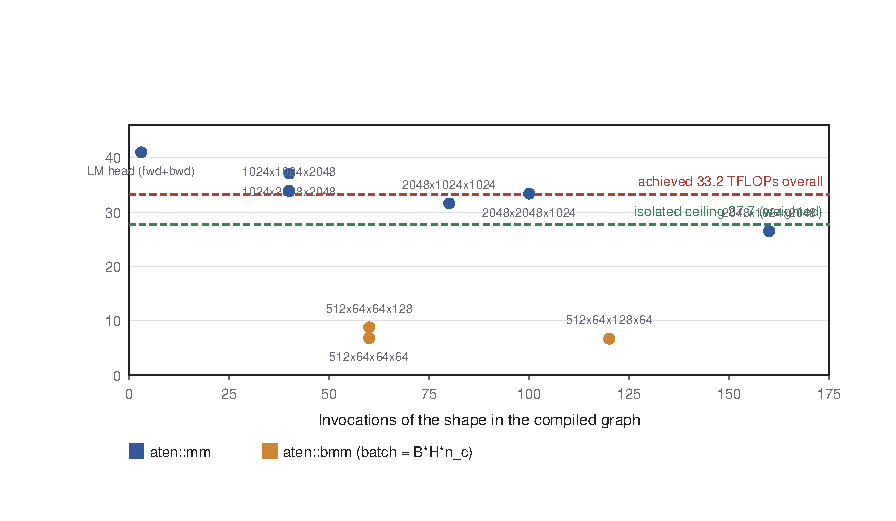
\includegraphics[width=\linewidth]{../figures/fig-gemm}
\caption{Matmul shapes issued by the compiled graph, with their in-place measured peaks and two reference lines.}
\label{fig:fig-gemm}
\end{figure}
\label{sec:en-eng-gemm}

\textbf{First, correct a wrong number that has been cited repeatedly.} The project's docs
claim ``11--21 TFLOPs for batch-1 shapes'', but the measurement is \textbf{26--42} (table
below). Using the batch-4 large-grid 42\,TFLOPs as a batch-1 ceiling manufactures a phantom
``40\% headroom''.

\code{scripts/gemm\_ceiling.py} computes an exact floor from two measured inputs: the shape
list comes directly from the compiled graph's dynamo counter \textbf{\code{aten\_mm\_info}}
(the \code{aten::mm} / \code{aten::bmm} calls that graph actually issued; the counts are
self-consistent with the LM head's three passes --- forward and backward --- at 1 each), and
each shape's peak is measured in place \textbf{without synchronising between calls} (otherwise
the 0.1\,ms chunkwise batched matmuls are drowned by sync overhead, under-reporting by
3--10$\times$).

\begin{center}\small
\captionof{table}{Matmul shapes issued by the compiled graph}
\begin{tabular}{@{}llrrr@{}}
\toprule
\textbf{Kind} & \textbf{Shape} & \textbf{Count} & \textbf{TFLOPs} & \textbf{Subtotal ms} \\
\midrule
mm & 2048$\times$1024$\times$2048 & 160 & 26.5 & 51.9 \\
mm & 2048$\times$2048$\times$1024 & 100 & 33.4 & 25.7 \\
mm & 2048$\times$1024$\times$1024 & 80 & 31.6 & 10.9 \\
mm & 1024$\times$2048$\times$2048 & 40 & 37.1 & 9.3 \\
mm & 1024$\times$1024$\times$2048 & 40 & 33.9 & 5.1 \\
mm & LM head, three passes & 1 each & 40--42 & 6.1 \\
bmm & 512$\times$64$\times$128$\times$64 & 120 & \textbf{6.7} & 9.7 \\
bmm & 512$\times$64$\times$64$\times$64 & 60 & \textbf{6.8} & 2.4 \\
bmm & 512$\times$64$\times$64$\times$128 & 60 & \textbf{8.8} & 3.7 \\
\bottomrule
\end{tabular}
\end{center}

(The bmm batch is $B{\cdot}H{\cdot}n_c$; the matrices are only 64$\times$64 or 64$\times$128, so
these reach only 6.7--8.8\,TFLOPs.)

\textbf{Conclusion:}

\begin{center}\small
\captionof{table}{Measured GEMM busy time against the shape-limited floor}
\begin{tabular}{@{}lr@{}}
\toprule
 & \textbf{ms/micro-step} \\
\midrule
Floor from the measured per-shape peaks & \textbf{124.6} \\
Profiler-measured GEMM busy time & \textbf{104.0} \\
Ratio & \textbf{0.83$\times$} \\
\bottomrule
\end{tabular}
\end{center}

\textbf{The measurement is below the isolated floor.} Put differently: it achieves
\textbf{33.2 TFLOPs} (3.457 TFLOP $\div$ 104\,ms), while the weighted shape peak is
\textbf{27.7 TFLOPs} (3.457 $\div$ 124.6\,ms) --- \textbf{already above the ceiling for these
shapes}. Both explanations (isolated measurement is conservative / the profiler buckets some
matmuls under Triton) point the same way: \textbf{there is no GEMM headroom left.}

The remaining 33.6\% non-GEMM is about 3500 Triton elementwise/reduction kernels at an average
of 34\,$\mu$s and roughly 350\,GB/s --- \textbf{running at DRAM bandwidth} (measured local copy
bandwidth 359--396\,GB/s). That part has an arithmetic intensity of only 0.5--2 FLOP/byte, is
\textbf{batch-invariant}, and can only improve by fusion --- which inductor has already
exhausted.

\subsection{Negative Results}
\label{sec:en-eng-neg}

\begin{center}\small
\captionof{table}{Negative results of the attempted optimizations}
\begin{tabular}{@{}>{\RaggedRight\arraybackslash}p{0.24\textwidth}>{\RaggedRight\arraybackslash}p{0.17\textwidth}>{\RaggedRight\arraybackslash}p{0.49\textwidth}@{}}
\toprule
\textbf{Attempt} & \textbf{Result} & \textbf{Reason} \\
\midrule
Fused linear $+$ cross-entropy (Liger-style [12]) &
\textbf{13\% slower} (batch 1) &
Numerically equivalent (bit-identical loss, gradient relative difference $\le$ 2.3e-4) and
saves 452.7\,MiB at batch 2, but the chunked loop requires
\code{torch.\_dynamo.disable} (otherwise the graph breaks and hangs), which loses compile
fusion \\
\code{\_head\_group\_norm} layout rewrite & \textbf{9.2\% slower} &
see Section~\ref{sec:en-arch-gn} \\
\code{torch.compile(\allowbreak mode="max-autotune-\allowbreak no-cudagraphs")} & \textbf{0\%} (662 vs 662) &
GEMM goes to external cuBLAS; autotune only affects Triton matmul templates \\
CUDA Graphs (\code{mode="reduce-overhead"}) & unusable &
hard conflict with gradient accumulation (the same graph runs 4 times with separate
backwards) \\
Log-depth (Hillis--Steele) scan & \textbf{2.8$\times$ slower} &
each round \code{torch.cat} materialises the whole $[B,H,n_c,d_k,d_v]$ \\
Physical batch 2 & memory-infeasible &
needs 9.81\,GiB reserved against an 8\,GB card \\
Layered gradient checkpointing & loses to C$'$ &
$K = 10/20 \rightarrow$ 816\,ms \\
\code{dataloader\_num\_\allowbreak workers} 0/2/4 & \textbf{0\%} &
the data pipeline is not the bottleneck \\
Removing \code{logits.float()} from the loss & \textbf{0\%} &
loss is bit-identical; the profiler's 3.9\% was an attribution artefact \\
dropout 0.1 $\rightarrow$ 0.0 & only 3.9\% saved &
and it changes the regularisation strength, so it is not worth it \\
\bottomrule
\end{tabular}
\end{center}

\section{Correctness Defects}
\label{sec:en-defects}

This section records three \textbf{silent} defects. What they have in common is:
\textbf{no error is raised, nothing crashes, and the logs look normal.}

\subsection{The \code{\_orig\_mod.} Prefix: No Checkpoint Would Load}
\label{sec:en-def-prefix}

\code{torch.compile(model)} returns an \code{OptimizedModule}, which places the original model
under an \code{\_orig\_mod} sub-module, so \textbf{every key} of \code{state\_dict()} gains an
\code{\_orig\_mod.} prefix.

In order to actually enable compilation (Section~\ref{sec:en-eng-compile}),
\code{retnet\_hf/train.py} assigned the compiled module to \code{trainer.model} and
\code{trainer.model\_wrapped} at the same time. HF's \code{save\_model} takes
\code{self.model.state\_dict()} --- \textbf{so every checkpoint written out carried the
prefix.}

And \code{RetNetForCausalLM.from\_pretrained} loads them \textbf{without error}: it discards
\code{\_orig\_mod.*} as ``unexpected keys'' and \textbf{randomly initialises} \code{blocks.*}
as ``missing keys''. The result:

\begin{lstlisting}[language=]
v13 final / rp / v10      365 keys, 0 prefixed    forward loss = 2.5767   logits finite
v14 checkpoint-10000      365 keys, 365 prefixed  forward loss = nan      all logits nan
\end{lstlisting}

On the evaluation side the symptom is \code{torch.multinomial} raising
\code{CUDA error: device-side assert triggered} --- \textbf{the root cause is simply not
reachable from the symptom}.

\textbf{Regression localisation}: v13's configuration had \code{compile=False}, v14 has
\code{compile=True}. The causal chain closes completely.

\textbf{The fix (three layers):}

\begin{enumerate}
\item \textbf{At the source}: stop wrapping the module and instead \textbf{replace
      \code{forward} in place} ---
      \code{trainer.model.forward = torch.compile(trainer.model.forward)}. Compilation still
      takes effect (measured 1.27 it/s, where eager drops to 0.45), while \code{state\_dict}
      stays clean, so \textbf{save, export and resume all become correct at once}.
\item \textbf{Rescue}: \code{scripts/strip\_compile\_prefix.py}, which strips the prefix in
      place and keeps a \code{.orig} backup.
\item \textbf{Gate}: \code{verify\_export()} checks the key names after every
      \code{save\_model} and raises a loud alarm;
      \code{scripts/check\_checkpoints.py} (binary, $O(1)$) and
      \code{scripts/verify\_checkpoint\_loads.py} (which really runs one forward pass) are
      available as a pre-load health check.
\end{enumerate}

All 17 historical checkpoints have been repaired and re-verified clean, and 6 bad backups have
been deleted.

\subsection{The Resume Path Never Worked}
\label{sec:en-def-resume}

\code{train.py} used to pass \code{resume\_from\_checkpoint=args.output\_dir}. But HF's
\code{Trainer.\_load\_from\_checkpoint} looks for weight files \textbf{directly} in the
directory it is given (\code{WEIGHTS\_NAME} / \code{SAFE\_WEIGHTS\_NAME} / \dots), while
\code{checkpoint-N} is a \textbf{subdirectory} of it, so it necessarily raises:

\begin{lstlisting}[language=]
ValueError: Can't find a valid checkpoint at checkpoints/retnet_272m_v14
\end{lstlisting}

This path had never actually been walked (the v14 log does not contain a single
\code{[restart]} line), so \code{auto\_restart\_max: 3} was an \textbf{empty promise}: the
moment a real crash happened, \code{run\_task.py} would restart, immediately raise the same
error again, and exit after three rounds. The scene is:

\begin{lstlisting}[language=]
[exit] rc=1
[restart] attempt 1/3 wait 3min
\end{lstlisting}

\textbf{The fix}: resolve the real checkpoint directory with
\code{transformers.trainer\_utils.\allowbreak get\_last\_checkpoint(\allowbreak output\_dir)}, pass that, and print
which one was chosen.

\begin{notebox}
This defect has a more dangerous adjacent form: once the checkpoints are repaired clean, resume
fails \textbf{the other way} --- HF does the \code{load\_state\_dict} with the compiled module
as the target, so all the clean keys are discarded as ``unexpected''. Without the fix of
Section~\ref{sec:en-def-prefix}, training would run \textbf{with the checkpoint's optimizer
state on top of the initial weights from \code{model\_dir}}, while the log prints only two
\code{missing/unexpected keys} warnings.
\end{notebox}

\subsection{An Equivalence Test That Compared a Function With Itself}
\label{sec:en-def-equiv}

\code{tests/test\_fast\_chunkwise.py} is designed as: reference implementation vs batched
implementation. But \code{modeling\_retnet.\_chunkwise\_retention} \textbf{forwards directly to
\code{chunkwise\_batched}} when the environment variable \code{RETNET\_FAST\_CHUNKWISE=1} ---
and the training environment always had that variable set.

\textbf{So the ``reference implementation'' was the function under test}, and the test always
reported ``bit-identical''. The table in \code{docs/15} \S2.3 claiming that ``all combinations
have bit-identical state'' \textbf{was never actually verified}.

\textbf{The fix}: add a \code{reference\_path} context manager that forces the sub-module
switch, and change the criterion from an \textbf{absolute} threshold to a \textbf{relative}
quantity (heads with $\gamma > 1$ amplify the state to $10^{13}$, which makes an absolute
threshold of $10^{-4}$ meaningless).

The real conclusion after the fix (all 15 combinations pass):

\begin{center}\small
\captionof{table}{Equivalence-test results}
\begin{tabular}{@{}>{\RaggedRight\arraybackslash}p{0.30\textwidth}rrr@{}}
\toprule
\textbf{gamma} & \textbf{out rel\_mean} & \textbf{out rel\_max} & \textbf{state rel\_max} \\
\midrule
Default init 0.9688--1.0000 & $\sim$1.4e-6 & 2.5e-7 -- 6.8e-7 & 2.4e-7 -- 7.0e-7 \\
\textbf{Real gate 0.6680--1.0117} & $\sim$8.1e-7 & 9.0e-7 -- 2.3e-6 & 5.1e-7 -- 2.1e-6 \\
Extreme 0.30--1.02 & $\sim$6.2e-7 & 3.1e-7 -- 3.6e-6 & 9.3e-7 -- 2.7e-6 \\
\bottomrule
\end{tabular}
\end{center}

\textbf{That is: the fast chunkwise path is not bit-equivalent but a relative-error
$10^{-6}$-level approximation} (the same order of magnitude before and after the change; the
closed-form scan did not make it worse).

\section{Evaluation}
\label{sec:en-eval}

\subsection{Benchmark Composition}

\begin{figure}[htbp]
\centering
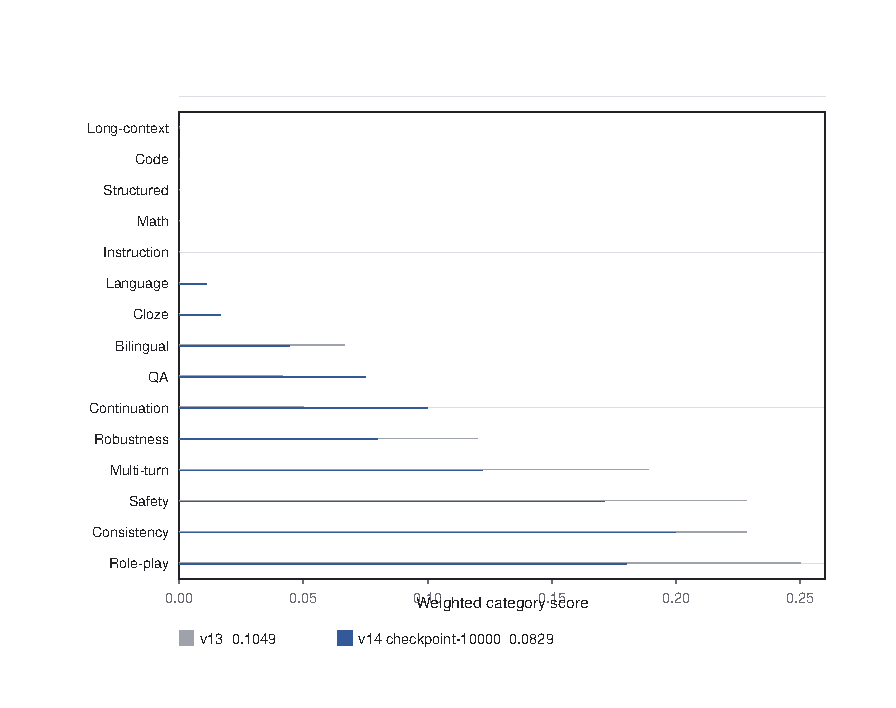
\includegraphics[width=\linewidth]{../figures/fig-bench-cats}
\caption{Per-category weighted score for v13 and v14 on the same item bank and seed.}
\label{fig:fig-bench-cats}
\end{figure}
\label{sec:en-eval-bench}

\code{bench/data/bench\_v3.jsonl}: \textbf{1,020 items / 15 categories / 136 families}, frozen
with a sha256. Decoding parameters $T = 0.7$, top\_k 40, top\_p 0.9, repetition\_penalty 1.1,
no\_repeat\_ngram 4, single seed 42.

\begin{center}\small
\captionof{table}{Benchmark composition by category}
\begin{tabular}{@{}lrlr@{}}
\toprule
\textbf{Category} & \textbf{Items} & \textbf{Category} & \textbf{Items} \\
\midrule
Cloze & 120 & Instruction following & 80 \\
QA & 120 & Consistency & 70 \\
Roleplay & 100 & Structured output & 60 \\
Multi-turn & 90 & Continuation & 60 \\
Language & 90 & Robustness & 50 \\
--- & --- & Long context & 50 \\
--- & --- & Bilingual & 45 \\
--- & --- & Safety & 35 \\
--- & --- & Code & 25 \\
--- & --- & Math & 25 \\
\bottomrule
\end{tabular}
\end{center}

\subsection{A Metric Defect That Had To Be Written Down}

\begin{figure}[htbp]
\centering
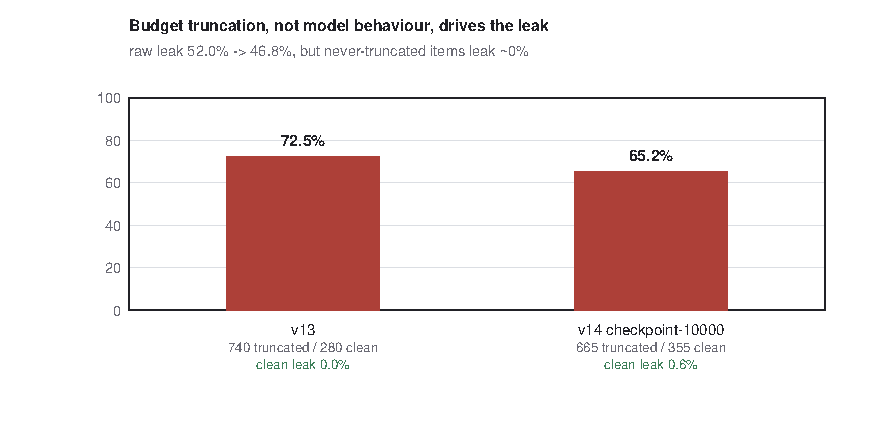
\includegraphics[width=\linewidth]{../figures/fig-truncation}
\caption{Truncation rate after splitting by budget truncation; never-truncated items leak at essentially zero.}
\label{fig:fig-truncation}
\end{figure}
\label{sec:en-eval-metric}

\textbf{Every item carries its own \code{max\_new}, measured to lie entirely in 16--160 (median
70)}, whereas the median CoT length in the training data is \textbf{570 tokens} (p10 377, p90
1072). \textbf{Giving a model whose median thought needs 570 tokens a budget of 16--160 tokens
makes closure physically impossible.}

Splitting the main run by whether it was budget-truncated (the criterion is
$n_{\text{new}} = \text{max\_new}$, which is exact for single-turn items):

\begin{center}\small
\captionof{table}{Leak rate split by budget truncation}
\begin{tabular}{@{}>{\RaggedRight\arraybackslash}p{0.36\textwidth}rrr@{}}
\toprule
\textbf{Subset} & \textbf{Items} & \textbf{Leak rate} & \textbf{Criterion passed} \\
\midrule
Single-turn, budget-truncated & \textbf{644} & \textbf{82.1\%} & 19 \\
Single-turn, \textbf{not truncated} & \textbf{235} & \textbf{0.0\%} & 47 \\
Multi-turn (conservative lower bound) & 133 & 0.8\% & 16 \\
\bottomrule
\end{tabular}
\end{center}

\textbf{All 530 items judged ``leaking'' fall inside the truncated subset, and the 243
never-truncated items leak not once.} The raw leak rate of 52.0\% is therefore \textbf{not a
number about the model}.

\begin{notebox}
This conclusion was first raised by \code{docs/17}. We re-verified it with an
\textbf{independent script} (\code{scripts/audit\_leak\_truncation.py}, read-only, joining the
raw jsonl to the item bank by id) and the \textbf{single-turn numbers agree exactly}
(644 / 82.1\%, 235 / 0.0\%, raw 52.0\%, \code{max\_new} 16--160).

The code side has been fixed: \code{bench/runner.py} now records \code{truncated} /
\code{max\_new} / \code{think\_leak\_untruncated}, \code{bench/analysis.py} emits the
truncation split (returning \code{None} rather than 0 when an old result file lacks the
\code{truncated} field), and \code{scripts/bench\_v3.py} gained a \code{--budget} override for
large-budget reruns.
\end{notebox}

\subsection{The Completed Comparison}
\label{sec:en-eval-compare}

\code{rp} / \code{v10} / \code{v13} / \code{v14 checkpoint-10000}, on the same 1,020-item bank,
the same seed 42 and the same decoding parameters:

\begin{center}\small
\captionof{table}{Comparison of the completed models}
\begin{tabular}{@{}>{\RaggedRight\arraybackslash}p{0.24\textwidth}rrrrr@{}}
\toprule
\textbf{Model} & \textbf{Weighted score} & \textbf{Raw leak} & \textbf{Truncated} &
\textbf{Untruncated} & \textbf{Untrunc.\ leak} \\
\midrule
\code{v13} & \textbf{0.1049} & 52.0\% & 740 (\textbf{72.5\%}) & 280 & \textbf{0.0\%} \\
\code{v14} \code{checkpoint-10000} & \textbf{0.0829} & 46.8\% & 665 (\textbf{65.2\%}) &
\textbf{355} & 0.6\% \\
\bottomrule
\end{tabular}
\end{center}

\begin{notebox}
The truncation criterion is uniformly $n_{\text{new}} \ge \text{max\_new} \times \text{turns}$
(exact for single-turn, a conservative lower bound for multi-turn); the 644 / 82.1\% of the
single-turn rows in Section~\ref{sec:en-eval-metric} is that same criterion restricted to the
single-turn subset. A looser rule without the $\times$turns factor would inflate the v13/v14
truncation rates to 76.2\% / 69.1\% respectively --- \textbf{this report does not use those
numbers}, and everything below uses the strict criterion.
\end{notebox}

Reading only those two rows suggests ``v14 got worse''. But they are \textbf{not} comparable
quantities --- the two models' ``untruncated subsets'' are \textbf{not the same items} (v13
stops only on the 280 easier-to-finish items, v14 stops on 355). An \textbf{intersection
comparison} is unavoidable:

\begin{center}\small
\captionof{table}{Intersection comparison}
\begin{tabular}{@{}>{\RaggedRight\arraybackslash}p{0.40\textwidth}rrrr@{}}
\toprule
\textbf{Subset} & \textbf{n} & \textbf{v13} & \textbf{v14} & \textbf{$\Delta$} \\
\midrule
All 1,020 items & 1020 & 0.0814 & 0.0716 & $-0.0098$ \\
\textbf{Intersection: untruncated for both} & \textbf{242} & \textbf{0.1942} & \textbf{0.1405} &
\textbf{$-0.0537$} \\
Only v13 untruncated & 38 & 0.211 & 0.105 & $-0.106$ \\
Only v14 untruncated & 113 & 0.097 & 0.044 & $-0.053$ \\
Both truncated & 627 & 0.027 & \textbf{0.048} & \textbf{$+0.021$} \\
\bottomrule
\end{tabular}
\end{center}

\textbf{Conclusions (with caveats):}

\begin{enumerate}
\item \textbf{v14's stopping behaviour really did improve} --- under the strict criterion the
      truncation rate falls 72.5\% $\rightarrow$ 65.2\% and the raw leak 52.0\% $\rightarrow$
      46.8\%. This agrees in direction with \code{docs/17}'s judgement that the firing rate is
      the real defect.
\item \textbf{But on the same items v14's accuracy is lower} (0.194 $\rightarrow$ 0.141, $-28\%$
      relative), and three of the four subsets agree in direction.
\item \textbf{The statistical power is insufficient.} On 242 items the binomial standard error
      at $p \approx 0.17$ is about 0.024 and the standard error of the difference about 0.034,
      so $\Delta = -0.054$ is about \textbf{1.6$\sigma$}. That \emph{suggests} a real
      regression but cannot settle it. Settling it needs multiple seeds (only seed 42 exists).
\end{enumerate}

\subsection{A Causal Hypothesis Awaiting Test: Restarting the LR After Annealing}
\label{sec:en-eval-hypothesis}

v14's configuration restarted a full cosine schedule \textbf{on v13 weights that had already
annealed to \code{min\_lr}}: the peak was $4\times10^{-5}$ while v13's final LR was
$1.1\times10^{-5}$ --- \textbf{a 3.6$\times$ jump}. (The rationale at the time is in the
comment in \code{tasks/v14\_272m\_2k\_cont.json}: ``the model had already annealed to
\code{min\_lr}; restarting at $1.1\times10^{-4}$ would break it first'', so the peak was
lowered to $4\times10^{-5}$.)

But two facts are observed together:

\begin{itemize}
\item v14's \textbf{training loss is lower} (2.4861 $\rightarrow$ 2.3686, against v13's 2.3707
      at step 10100);
\item v14's \textbf{benchmark accuracy is lower} (0.194 $\rightarrow$ 0.141 on the
      intersection).
\end{itemize}

``Falling training loss with falling task accuracy'' is the classic signature of
\textbf{overfitting / catastrophic forgetting}, and ``restarting the LR after annealing'' is a
known trigger for it.

\textbf{We have not verified this}; it is listed in Section~\ref{sec:en-limits} as the first
experiment for the next round: same data, same step span, but \textbf{without restarting the
LR} (continuing from $1.1\times10^{-5}$), to see whether the intersection accuracy returns to
the v13 level.

\section{Limitations and Future Work}
\label{sec:en-limits}

\begin{enumerate}
\item \textbf{Capacity.} The CoT capability threshold recorded in \code{docs/04} is 0.5--1B
      parameters, and 272M is below it. Long-context retrieval (fetching one fact across
      1.2K tokens) and multi-step arithmetic are stably zero on 272M, and they are also zero
      for v10 (0.28 epoch) --- these two \textbf{do not look like a training-volume problem}.
      But the converse cannot be excluded either: this model has \textbf{never} seen the
      552M-token corpus once through (v13 reached 18.5\%; v14 accumulates about 92.6\% by step
      50,000). Neither direction currently has decisive evidence.
\item \textbf{Memory.} Physical batch 2 requires 9.81\,GiB reserved, which does not fit on an
      8\,GB card; activations are 59\% of peak memory and are the only movable part.
      \textbf{The 8\,GB limit constrains throughput, not capacity} --- per the estimate in
      \code{docs/16} (\textbf{not independently verified}; see the reference-reliability note
      below), the same card fits roughly 700M parameters once gradient checkpointing is
      enabled, at a cost of $3.3\times$ per step.
\item \textbf{Train/inference inconsistency.} Training takes the chunkwise path while
      \code{generate()}'s prefill takes the parallel path; the two are not numerically
      identical, and there is currently \textbf{no guard} for it.
\item \textbf{Unverified citations.} See the annotations in the reference list.
\item \textbf{An unresolved capability regression.} v14 is 28\% below v13 on the
      truncation-corrected intersection (0.194 $\rightarrow$ 0.141, about 1.6$\sigma$). Only a
      single seed exists, so \textbf{the statistical power is insufficient to conclude}, but
      the direction is consistent and is accompanied by the typical ``falling training loss
      with falling task accuracy'' signature. The leading hypothesis awaiting test is the
      \textbf{restart of the learning rate after annealing} of
      Section~\ref{sec:en-eval-hypothesis}.
\item \textbf{One unexplained observation.} v13's loss near step 10020 is $\approx$ 2.47,
      while v14 at the same position is 2.4092 --- a gap of about 0.06, far larger than the
      measured chunk-64/128 single-batch difference of 2.4e-7. The two should have seen the
      same data window (v14 was rolled back to \code{checkpoint-10000} and rerun).
      \textbf{We have not got to the bottom of it}; candidate explanations include the
      dataloader's skip semantics, and the effect of the first leg's abnormal termination on
      the RNG state.
\end{enumerate}

\section{Conclusion}
\label{sec:en-concl}

On a single 8\,GB consumer GPU the per-optimization-step time of RetNet-272M falls from
\textbf{2176\,ms to 662\,ms (3.29$\times$)}, with every conclusion built on wall-clock
measurement of the real \code{Trainer} path and on numerical-equivalence tests. The main
algorithmic contribution of this report is a \textbf{closed-form state scan}: exploiting the
fact that the per-chunk decay is constant across the loop, it replaces the $n_c$-step serial
recurrence with a single batched matrix multiplication, cutting each layer from 1127\,$\mu$s
to 190\,$\mu$s while the relative error stays at the level of fp32 accumulation noise.

Three methodological conclusions matter more than the numbers:

\begin{enumerate}
\item \textbf{A claim that ``we are at the limit'' must be traceable to its measurement
      conditions.} The project inferred ``removing kernels is useless'' from a
      battery-measured ``20.8\% GPU idle'', yet on AC the true occupancy is 94\% --- and both
      real optimizations (8\% combined) are precisely kernel removal.
\item \textbf{The shape of the bottleneck changes.} Before the optimizations it was launch
      count; after them it is the shape-limited GEMM ceiling. The same model on the same
      hardware, and a completely different answer.
\item \textbf{Silent correctness defects cost more than performance problems.} All three
      defects reported here (checkpoints that would not load, a resume path that never
      worked, an equivalence test that compared a function with itself) raised no error. They
      survived this long only because \textbf{nobody ever actually loaded those checkpoints}.
\end{enumerate}

\startappendix
\section{Appendix A: Reproduction}
\label{sec:en-appA}

The command block is reproduced verbatim from the source (only the \code{\#} comments have
been translated):

\begin{lstlisting}[language=PowerShell]
# 1) Step-time comparison (real Trainer path, AC power)
$env:RETNET_FAST_CHUNKWISE='1'
python scripts\bench_trainer.py --model_dir checkpoints\retnet_272m_rp `
    --data_dir data_cache\chat_pack_v13 --max_steps 70 --batch_size 1 `
    --grad_accum 4 --chunk_size 128 --compile --no_grad_checkpoint `
    --optim adamw_bnb_8bit --warm_skip 25

# 2) chunk sweep (only meaningful after fixing config.chunk_size)
#    replace --chunk_size with 64 / 128 / 256 in turn

# 3) Kernel-level attribution (chrome trace -> aggregate by CUDA kernel)
python scripts\profile_kernels.py --batch_size 1 --grad_accum 4 --chunk_size 128 `
    --compile --no_grad_checkpoint --optim adamw_bnb_8bit --steps 10 --active 3

# 4) How far GEMM is from the ceiling
python scripts\gemm_ceiling.py --reps 25

# 5) Equivalence regression (mandatory)
python tests\test_fast_chunkwise.py      # 15 combinations
python tests\test_head_group_norm.py
python tests\test_control.py             # external flag control, 22 cases

# 6) Checkpoint health check
python scripts\check_checkpoints.py --root checkpoints          # key names, O(1)
python scripts\verify_checkpoint_loads.py --ckpt <dir>          # really run one forward

# 7) Leak rate / truncation split (read-only, no GPU needed)
python scripts\audit_leak_truncation.py --run logs\bench_v3\v13.T0.7_s1.jsonl --by-cat

# 8) Evaluation
python scripts\bench_v3.py --models "m=checkpoints/retnet_272m_v14/checkpoint-10000" `
    --tokenizer data_cache/chat_pack_v13/bpe_tokenizer.json --seeds 42 `
    --out logs\bench_v3 --tag <tag>
# Large-budget rerun (deciding "will it close" needs a bigger budget, see Section 8.2)
#    append --budget 1024

# 9) Training (laptop; schtasks detaches it from SSH)
schtasks /create /tn RetNet_v14r /tr "cmd /c C:\Users\Ayaka\RetNet\tasks\start_v14_resume.bat" `
    /sc once /st 23:59 /f
schtasks /run /tn RetNet_v14r
# Graceful stop (do not taskkill):
python run_task.py --ctrl next-checkpoint
\end{lstlisting}

\section{Appendix B: Key Code}
\label{sec:en-appB}

The snippets below keep the original code and the original Chinese comments (the shared
preamble supports CJK inside \code{lstlisting}).

\subsection{Closed-Form State Scan (\code{retnet\_hf/retention\_fast.py})}

\begin{lstlisting}[language=Python]
# (2) 闭式扫描：decay = chunk_decay 在循环里是常量，于是
#     S_prev[i] = d^i·state + Σ_{j<i} d^(i-1-j)·U_j
# 这正是对 T[h,i,j] = d_h^(i-1-j)（下三角）的一次批量矩阵乘。
# 多出来的一行 i=nc 恰好是 new_state。所有指数非负 → 无 γ^-j 溢出。
log_d = torch.log(gamma.to(device=dev, dtype=torch.float32)) * float(chunk_size)
idx = torch.arange(nc + 1, device=dev)
expo_t = idx[:, None] - torch.arange(nc, device=dev)[None, :] - 1
valid_t = expo_t >= 0
T = torch.exp(log_d[:, None, None] * expo_t.clamp_min(0).to(torch.float32)[None])
T = torch.where(valid_t[None], T, torch.zeros((), device=dev, dtype=torch.float32))
T = T.to(q.dtype)                                          # [H, nc+1, nc]

U_flat = U.reshape(B, H, nc, kd * vd)
S_all = torch.matmul(T[None], U_flat)                      # [B,H,nc+1,kd*vd]
if has_state:
    t_state = torch.exp(log_d[:, None] * idx.to(torch.float32)[None]).to(q.dtype)
    S_all = S_all + t_state[None, :, :, None] * state.reshape(B, H, 1, kd * vd)

S_prev = S_all[:, :, :nc].reshape(B, H, nc, kd, vd)
new_state = S_all[:, :, nc].reshape(B, H, kd, vd)
\end{lstlisting}

\subsection{Log-Space Decay Mask (\code{retnet\_hf/retention\_fast.py})}

\begin{lstlisting}[language=Python]
causal, expo, relf = _index_tables(chunk_size, device)
g = gamma.to(device=device, dtype=torch.float32)
log_gamma = torch.log(g)

# exp(log γ · delta)：两个方向都正确饱和。绝不能写成 γ^i · γ^-j ——
# 本模型 γ 最小 0.668，0.668^-255 = 1e44 > 3.4e38 → Inf → NaN。
inner_mask = torch.exp(log_gamma[:, None, None] * expo[None])
inner_mask = torch.where(causal, inner_mask,
                         torch.zeros((), device=device, dtype=torch.float32))

pow1d = torch.exp(log_gamma[:, None] * relf[None, :])     # [H,C] = γ^j
cross_decay = pow1d * g[:, None]                          # γ^(j+1)
value_decay = pow1d.flip(-1)                              # γ^(C-1-j)
chunk_decay = pow1d[:, -1] * g                            # γ^C
\end{lstlisting}

\subsection{In-Place Compilation (\code{retnet\_hf/train.py})}

\begin{lstlisting}[language=Python]
# 就地替换 forward，**不要**把模型包成 OptimizedModule —— 那会给 state_dict
# 的每一个键加 `_orig_mod.` 前缀，让保存的检查点静默变成随机模型。
compiled_fwd = torch.compile(trainer.model.forward, backend="inductor")
trainer.model.forward = compiled_fwd
\end{lstlisting}

\subsection{Export Self-Check (\code{retnet\_hf/train.py})}

\begin{lstlisting}[language=Python]
def verify_export(path) -> bool:
    """safetensors 的键里不能有 `_orig_mod.`，否则 from_pretrained 会静默随机初始化。"""
    ...
    bad = [k for k in keys if k.startswith("_orig_mod.")]
    if bad:
        print(f"[verify] |$\times$| 导出里有 {len(bad)}/{len(keys)} 个键带 _orig_mod. 前缀 —— "
              f"这个检查点用 from_pretrained 加载会**静默变成随机模型**。")
        return False
    print(f"[verify] |$\checkmark$| 导出键名干净（{len(keys)} 个），可直接 from_pretrained")
\end{lstlisting}

\subsection{Resume Path (\code{retnet\_hf/train.py})}

\begin{lstlisting}[language=Python]
if args.resume:
    from transformers.trainer_utils import get_last_checkpoint
    last = get_last_checkpoint(args.output_dir)
    if last is None:
        raise SystemExit(f"--resume 但 {args.output_dir} 里找不到 checkpoint-* 子目录。")
    print(f"[resume] 从 {last} 续训（优化器 / LR 调度器状态由 HF 一并恢复）", flush=True)
    resume_arg = last
else:
    resume_arg = False
trainer.train(resume_from_checkpoint=resume_arg)
\end{lstlisting}

\section{Appendix C: External Flag Control (\code{retnet\_hf/control.py})}
\label{sec:en-appC}

Stopping a running training job used to require \code{taskkill}, and even the order had to be
right (\code{run\_task.py} does
\code{if rc != 0 and attempts < auto\_restart\_max: restart} --- killing \code{train.py}
directly yields \code{rc=1} and gets the job restarted). A flag lets training exit
\textbf{gracefully at a step boundary}:

\begin{itemize}
\item \code{run} --- continue; the default, also used to clear an instruction.
\item \code{stop} --- stop after the current optimization step, without waiting for a
      checkpoint.
\item \code{next-checkpoint} --- stop after the next checkpoint write; the checkpoint is
      flushed to disk before the exit.
\item \code{save} --- write a checkpoint immediately, then continue.
\end{itemize}

\textbf{The correctness basis}: in \code{transformers/trainer.py}'s
\code{\_inner\_training\_loop}, line 2755 \code{on\_step\_end} precedes line 2756
\code{\_maybe\_log\_save\_evaluate} (checkpoint $+$ evaluation) and the \code{break} is at
line 2772. Setting \code{control.should\_training\_stop} inside \code{on\_step\_end} therefore
\textbf{saves the checkpoint before exiting} --- which is exactly why ``stop after the next
checkpoint'' can be written correctly.

\code{stop} and \code{next-checkpoint} are \textbf{sticky} (the flag is not cleared after it
fires), so that \code{run\_task.py} can tell ``stopped on external request'' apart from
``crashed, should be restarted''.

\section{Appendix D: Defect Summary}
\label{sec:en-appD}

\begin{center}\small
\setlength{\tabcolsep}{4pt}
\begin{tabular}{@{}>{\RaggedRight\arraybackslash}p{0.03\textwidth}>{\RaggedRight\arraybackslash}p{0.15\textwidth}>{\RaggedRight\arraybackslash}p{0.20\textwidth}>{\RaggedRight\arraybackslash}p{0.21\textwidth}>{\RaggedRight\arraybackslash}p{0.27\textwidth}@{}}
\toprule
\textbf{\#} & \textbf{Defect} & \textbf{Symptom} & \textbf{Why silent} & \textbf{Fix} \\
\midrule
1 & \code{\_orig\_mod.} prefix & loss $=$ nan after loading a checkpoint &
\code{from\_pretrained} silently drops the unexpected keys &
in-place forward compile $+$ strip tool $+$ export self-check \\
2 & Resume path & \code{Can't find a valid checkpoint} &
the path was never actually exercised & \code{get\_last\_checkpoint()} \\
3 & Self-comparing equivalence test & always reports ``bit-identical'' &
the environment variable forwards the reference to the function under test &
\code{reference\_path} context plus a relative criterion \\
4 & HF loss normalisation & loss inflated \code{accum}$\times$ &
it only fires when \code{accum > 1} & \code{accepts\_loss\_kwargs = False} \\
5 & \code{config.\allowbreak chunk\_size} & the config is ignored & nothing errors &
fall back to the config in \code{forward} \\
6 & \code{eval\_batch\_\allowbreak mult} & the config is ignored and evaluation is 2.4$\times$ slower &
nothing errors & wire it into \code{train.py} \\
7 & \code{torch.compile} silently ineffective &
the log says applied, the speedup is 0\% &
inductor compiles lazily plus the wrapping is misplaced &
an explicit \code{import triton} $+$ in-place forward replacement \\
8 & \code{save\_total\_\allowbreak limit} &
the config says 4, the actual value is 3, and \code{checkpoint-\allowbreak 10000} was rotated away &
the deletion line is \code{logger.info} while \code{transformers} defaults to \code{WARNING} &
wire it into \code{train.py}; the criterion is to read \code{training\_args.bin}, not the config JSON \\
\bottomrule
\end{tabular}
\end{center}

\backmattersection{References}\label{sec:refs}

\textbf{[1]} Y. Sun, L. Dong, S. Huang, S. Ma, Y. Xia, X. Zhang, J. Li, F. Wei. *Retentive Network: A Successor to Transformer for Large Language Models.* arXiv:2307.08621, 2023.

\textbf{[2]} S. Yang, B. Wang, Y. Shen, R. Panda, Y. Kim. *Gated Linear Attention Transformers with Hardware-Efficient Training.* arXiv:2312.06635, 2023.

\textbf{[3]} A. Katharopoulos, A. Vyas, N. Pappas, F. Fleuret. *Transformers are RNNs: Fast Autoregressive Transformers with Linear Attention.* arXiv:2006.16236, 2020.

\textbf{[4]} A. Gu, T. Dao. *Mamba: Linear-Time Sequence Modeling with Selective State Spaces.* arXiv:2312.00752, 2023.

\textbf{[5]} T. Dao, A. Gu. *Transformers are SSMs: Generalized Models and Efficient Algorithms Through Structured State Space Duality.* arXiv:2405.21060, 2024.

\textbf{[6]} S. Yang, B. Wang, Y. Zhang, Y. Shen, Y. Kim. *Parallelizing Linear Transformers with the Delta Rule over Sequence Length.* arXiv:2406.06484, 2024.

\textbf{[7]} S. Yang, J. Kautz, A. Hatamizadeh. *Gated Delta Networks: Improving Mamba2 with Delta Rule.* arXiv:2412.06464, 2024.

\textbf{[8]} S. De, S. L. Smith, A. Fernando, A. Botev, G. Cristian-Muraru, A. Gu, et al. *Griffin: Mixing Gated Linear Recurrences with Local Attention for Efficient Language Models.* arXiv:2402.19427, 2024.

\textbf{[9]} B. Peng, E. Alcaide, Q. Anthony, A. Albalak, S. Arcadinho, et al. *RWKV: Reinventing RNNs for the Transformer Era.* arXiv:2305.13048, 2023.

\textbf{[10]} T. Dao, D. Y. Fu, S. Ermon, A. Rudra, C. Ré. *FlashAttention: Fast and Memory-Efficient Exact Attention with IO-Awareness.* arXiv:2205.14135, 2022.

\textbf{[11]} T. Dettmers, M. Lewis, S. Shleifer, L. Zettlemoyer. *8-bit Optimizers via Block-wise Quantization.* arXiv:2110.02861, 2021.

\textbf{[12]} P.-L. Hsu, Y. Dai, V. Kothapalli, Q. Song, S. Tang, S. Zhu, et al. *Liger Kernel: Efficient Triton Kernels for LLM Training.* arXiv:2410.10989, 2024.

\textbf{[13]} I. Loshchilov, F. Hutter. *Decoupled Weight Decay Regularization.* arXiv:1711.05101, 2017.

\textbf{[14]} I. Loshchilov, F. Hutter. *SGDR: Stochastic Gradient Descent with Warm Restarts.* arXiv:1608.03983, 2016.

\textbf{[15]} P. Micikevicius, S. Narang, J. Alben, G. Diamos, E. Elsen, et al. *Mixed Precision Training.* arXiv:1710.03740, 2017.

\textbf{[16]} B. Zhang, R. Sennrich. *Root Mean Square Layer Normalization.* arXiv:1910.07467, 2019.

\textbf{[17]} Y. Wu, K. He. *Group Normalization.* arXiv:1803.08494, 2018.

\textbf{[18]} T. Chen, I. Goodfellow, J. Shlens. *Net2Net: Accelerating Learning via Knowledge Transfer.* arXiv:1511.05641, 2015.

\textbf{[19]} C. Chen, Y. Yin, L. Shang, X. Jiang, Y. Qin, F. Wang, et al. *bert2BERT: Towards Reusable Pretrained Language Models.* arXiv:2110.10329, 2021.

\textbf{[20]} J. Hoffmann, S. Borgeaud, A. Mensch, E. Buchatskaya, T. Cai, et al. *Training Compute-Optimal Large Language Models.* arXiv:2203.15556, 2022.

\textbf{[21]} DeepSeek-AI. *DeepSeek-R1: Incentivizing Reasoning Capability in LLMs via Reinforcement Learning.* arXiv:2501.12948, 2025.

\textbf{[22]} W. Merrill, A. Sabharwal. *The Illusion of State in State-Space Models.* arXiv:2404.08819, 2024.

\textbf{[23]} O. Lieber, B. Lenz, H. Bata, G. Cohen, J. Osin, I. Dalmedigos, et al. *Jamba: A Hybrid Transformer-Mamba Language Model.* arXiv:2403.19887, 2024.

\textbf{[24]} P. Tillet, H.-T. Kung, D. Cox. *Triton: An Intermediate Language and Compiler for Tiled Neural Network Computations.* MAPL@PLDI, 2019.

\reportrule

\backmattersection{Reference Reliability Note}

The following entries are quoted from internal project surveys and were \textbf{not independently verified}; confirm them before relying on them:

\begin{itemize}
  \item \textbf{arXiv:2507.06457} (a 340M$\times$20B controlled study of the linear:full attention ratio and recall) and \textbf{arXiv:2605.16640} (chain-of-thought solvability of hybrid vs pure linear), both cited by \code\{docs/18\}. The identifier form of the latter is suspicious (2605 would be May 2026) and should be checked.
  \item \code\{docs/18\}'s quantitative claim that four linear mechanisms differ by only 1.6\% downstream at 340M/20B.
  \item \code\{docs/16\}'s estimate that 8\textbackslash{},GB fits 54 layers $\approx$ 700M parameters under gradient checkpointing.
\end{itemize}

For references \textbf{[1]--[24]}, every entry that carries a specific numeric conclusion has that conclusion \textbf{measured by this project itself} (the provenance is in the body of the report); the literature is cited only to identify the origin of the method.

\end{document}
